\documentclass[a4paper,14pt]{extarticle}
\usepackage[utf8]{inputenc}
\usepackage[T1]{fontenc}
\usepackage[russian]{babel}
\usepackage{indentfirst}
\usepackage{geometry}
\usepackage{fontspec}
\usepackage{wrapfig}
\usepackage[explicit]{titlesec}
\usepackage{longtable}
\usepackage{graphicx}
\usepackage{float}
\usepackage{array}
\usepackage[
    figurename=Рисунок,
    labelsep=endash,
]{caption}
\usepackage{hyperref}
\usepackage{tocloft}

\geometry{
    left=30mm,
    top=20mm,
    bottom=20mm,
    right=15mm,
}

\setmainfont{Times New Roman}

\hypersetup{
    colorlinks=true,
    linkcolor=black,
    urlcolor=blue,
}

\titleformat{\section}
{\normalfont}{\bfseries \thesection.}{4pt}{\bfseries #1}

\titleformat{\subsection}
{\normalfont}{\bfseries \thesubsection.}{4pt}{\bfseries #1}

\renewcommand{\baselinestretch}{1.5}

\captionsetup{width=\textwidth}
\captionsetup[table]{singlelinecheck=off,justification=raggedright}

\renewcommand{\cftsecleader}{\cftdotfill{\cftdotsep}}
\renewcommand{\cftsecaftersnum}{.}%

\addto\captionsrussian{\renewcommand{\contentsname}{Содержание\hfill}}
\renewcommand{\cfttoctitlefont}{\hfill\bfseries}
\renewcommand{\cftaftertoctitle}{\hfill}

\setlength\LTcapwidth{\textwidth}
\setlength\LTleft{0pt}
\setlength\LTright{0pt}

\begin{document}

\begin{titlepage}
    \vspace{0pt plus2fill}
    \noindent

    \vspace{0pt plus6fill}
    \begin{center}
        Министерство образования и науки

        федеральное государственное автономное образовательное учреждение высшего образования

        <<Национальный исследовательский университет ИТМО>>

        Факультет инфокоммуникационных технологий

        \vspace{0pt plus8fill}

        Отчет по курсу: \textbf{<<Базы данных>>}

        \textbf{<<Интернет площадка креативных товаров>>}
    \end{center}

    \vspace{0pt plus8fill}
    \begin{flushright}
        Выполнили: \\
        Швалов Даниил Андреевич \\
        Осыченко Арсений Дмитриевич \\
        Богданов Михаил Александрович \\
        Ларичева Дарья Кирилловна \\
        Карагодин Максим Александрович

        Группа: К32211

        Проверила: \\
        Осетрова Ирина Станиславовна
    \end{flushright}

    \vspace{0pt plus5fill}
    \begin{center}
        Санкт-Петербург \\ 2022
    \end{center}
\end{titlepage}

\setcounter{page}{2}

\tableofcontents
\newpage

\section{Введение}

Уже достаточно долгое время интернет-площадки для покупки и продажи вещей пользуются огромной популярностью. На рынке существует множество площадок, предоставляющих сервис для продажи различных видов товаров.

<<Креатистор>> -- это интернет-площадка для креативных людей, интересных идей и уникальных товаров. На рынке существует множество различных магазинов креативных товаров. Однако мы готовы предложить сервис, отличный от существующих.

Мы, равно как наши конкуренты, не покупаем и не продаем товары. Наша компания предоставляем площадку, на которой продавцы находят своих покупателей, а покупатели получают возможность приобрести креативные товары. Однако, в отличии от остальных площадок мы ориентированы не на масс-маркет, а на нишу людей, интересующимся креативными вещами.

\section{Цели}

Целью данной лабораторной работы является разработка логической схемы базы данных для интернет-площадки по продаже креативных вещей.

\section{Задачи}

Для достижения поставленной цели необходимо выполнить следующие задачи:
\begin{itemize}
    \item анализ предметной области;
    \item анализ существующих аналогов;
    \item анализ пользовательских возможностей;
    \item выделение основных сущностей;
    \item определение связей между сущностями;
    \item создание графических схем базы данных.
\end{itemize}

\section{Концепт интернет-площадки}

Интернет площадка <<Креатистор>> достаточно сильно похожа на существующие аналоги. Это не удивительно, поскольку достаточно сложно придумать что-то новое в хорошо освоенной сфере. Однако у нашей площадки есть некоторые особенности, которые отличают нас от остальных. Основная особенность заключается в том, что наша площадка ориентирована на креативных людей, предлагающих креативные товары.

Разберем эту идею подробнее, а точнее, каким образом мы собираемся ее реализовать. В первую очередь рассмотрим то, каким способом мы собираемся оставаться площадкой с креативными товарами. Наш способ -- модерация. Именно модерация -- это первое, что отличает по части реализации нашу платформу от своих аналогов. Поскольку наша площадка стремится быть местом только с креативными товарами, нам необходимо проверять каждое объявление. Это позволит избежать продажи некачественного товара, а также товаров широкого потребления.

Еще одно отличие -- это поддержания почти полного равноправия на площадке. Во многих сервисах по продаже товаров предусмотрены способы по продвижению своих товаров. Так, например, это может быть поднятие объявления в поиске или закрепление его. На нашей площадке этого не предусмотрено. Мы считаем, что объявления должны выдаваться только в порядке качества заполнения информации о товаре: чем подробнее, точнее и качественнее написано описание товара, тем более вероятно, что именно этот товар попадется в поиске. В то же время, благодаря модерации будут исключены случаи подкрутки описания под поисковые алгоритмы.

Однако тут же возникает вопрос о монетизации платформы. Именно из-за монетизации на нашей платформе только почти равноправие. Особенностью нашей платформы является то, что только пользователи с подпиской могут добавлять свои товары. Другими словами, чтобы добавить свой товар на нашу платформу, пользователю необходимо приобрести подписки. Однако это никак не распространяется на просмотр и поиск объявлений: даже незарегистрированный пользователь может искать и просматривать объявления на нашей платформе.

Итого, наша платформа имеет следующие аспекты, отличающие нас от наших конкурентов:
\begin{itemize}
    \item модерация товаров;
    \item отсутствие методов продвижения товаров;
    \item подписочная система.
\end{itemize}

\section{Сравнение с аналогами}

В отличии от конкурентов, наша площадка предлагает одинаковую и справедливую для всех систему выставления товара. Хотя и для размещения объявления требуется приобрести подписку, в отличии от остальных сервисов, все продавцы находятся в равных условиях, что позволяет только начинающим в своем деле людям, у которых нет большого количества средств, конкурировать с остальными продавцами только за счет качества свое товара. Сравнение функциональных возможностей представлено в таблице \ref{tab:comparison}.

\begin{center}
    \begin{longtable}{|>{\centering\arraybackslash}m{3.5cm}|>{\centering\arraybackslash}m{2.7cm}|>{\centering\arraybackslash}m{2.7cm}|>{\centering\arraybackslash}m{2.7cm}|>{\centering\arraybackslash}m{2.7cm}|}
        \caption{Сравнительная таблица аналогов}
        \label{tab:comparison}
        \\
        \hline
        \textbf{Функциал / Платформа}   & \textbf{Креатистор} & \textbf{Авито}  & \textbf{Юла}    & \textbf{Фарпост} \\
        \hline
        \textbf{Чат с продавцом}        & Да                  & Да              & Да              & Да               \\
        \hline
        \textbf{Избранные товары}       & Да                  & Да              & Да              & Да               \\
        \hline
        \textbf{Тип модерации}          & Премодерация        & Постмодерация   & Постмодерация   & Постмодерация    \\
        \hline
        \textbf{Подписочная система}    & Да                  & Да              & Да              & Нет              \\
        \hline
        \textbf{Контактные данные}      & Да                  & Да              & Да              & Да               \\
        \hline
        \textbf{Поиск по названию}      & Да                  & Да              & Да              & Да               \\
        \hline
        \textbf{Поиск по тегам}         & Да                  & Нет             & Нет             & Нет              \\
        \hline
        \textbf{Поиск по категориям}    & Нет                 & Да              & Да              & Да               \\
        \hline
        \textbf{Создание объявления}    & По подписке         & При регистрации & При регистрации & При регистрации  \\
        \hline
        \textbf{Продвижение объявления} & Нет                 & Да              & Да              & Да               \\
        \hline
        \textbf{Платежная система}      & Нет                 & Да              & Да              & Да               \\
        \hline
        \textbf{Доставка}               & Нет                 & Да              & Да              & Да               \\
        \hline
    \end{longtable}
\end{center}


\section{Пользовательские возможности}

В этом разделе описан основной функционал, предоставленный пользователю. При взаимодействии с площадкой пользователь может:
\begin{itemize}
    \item создавать, входить в личный аккаунт;
    \item просматривать и искать товары;
    \item приобретать подписку, расширяющую доступный функционал;
    \item создавать и редактировать товары;
    \item добавлять товары в избранное;
    \item оставлять отзывы на продавцов;
    \item общаться с продавцом с помощью чата.
\end{itemize}
Рассмотрим каждый функционал поподробнее.

\subsection{Просмотр и поиск товаров}

Первое, с чем будет взаимодействовать пользователь -- это товары, который он присматривает себе. Кроме привычной ленты товаров, наша платформа предлагает поиск по товарам. На нем сделан особый акцент, потому что он несколько отличается от привычного поиска на торговых площадках. Схема поиска товаров показана на рисунке \ref{fig:search}.

\begin{figure}[H]
    \centering
    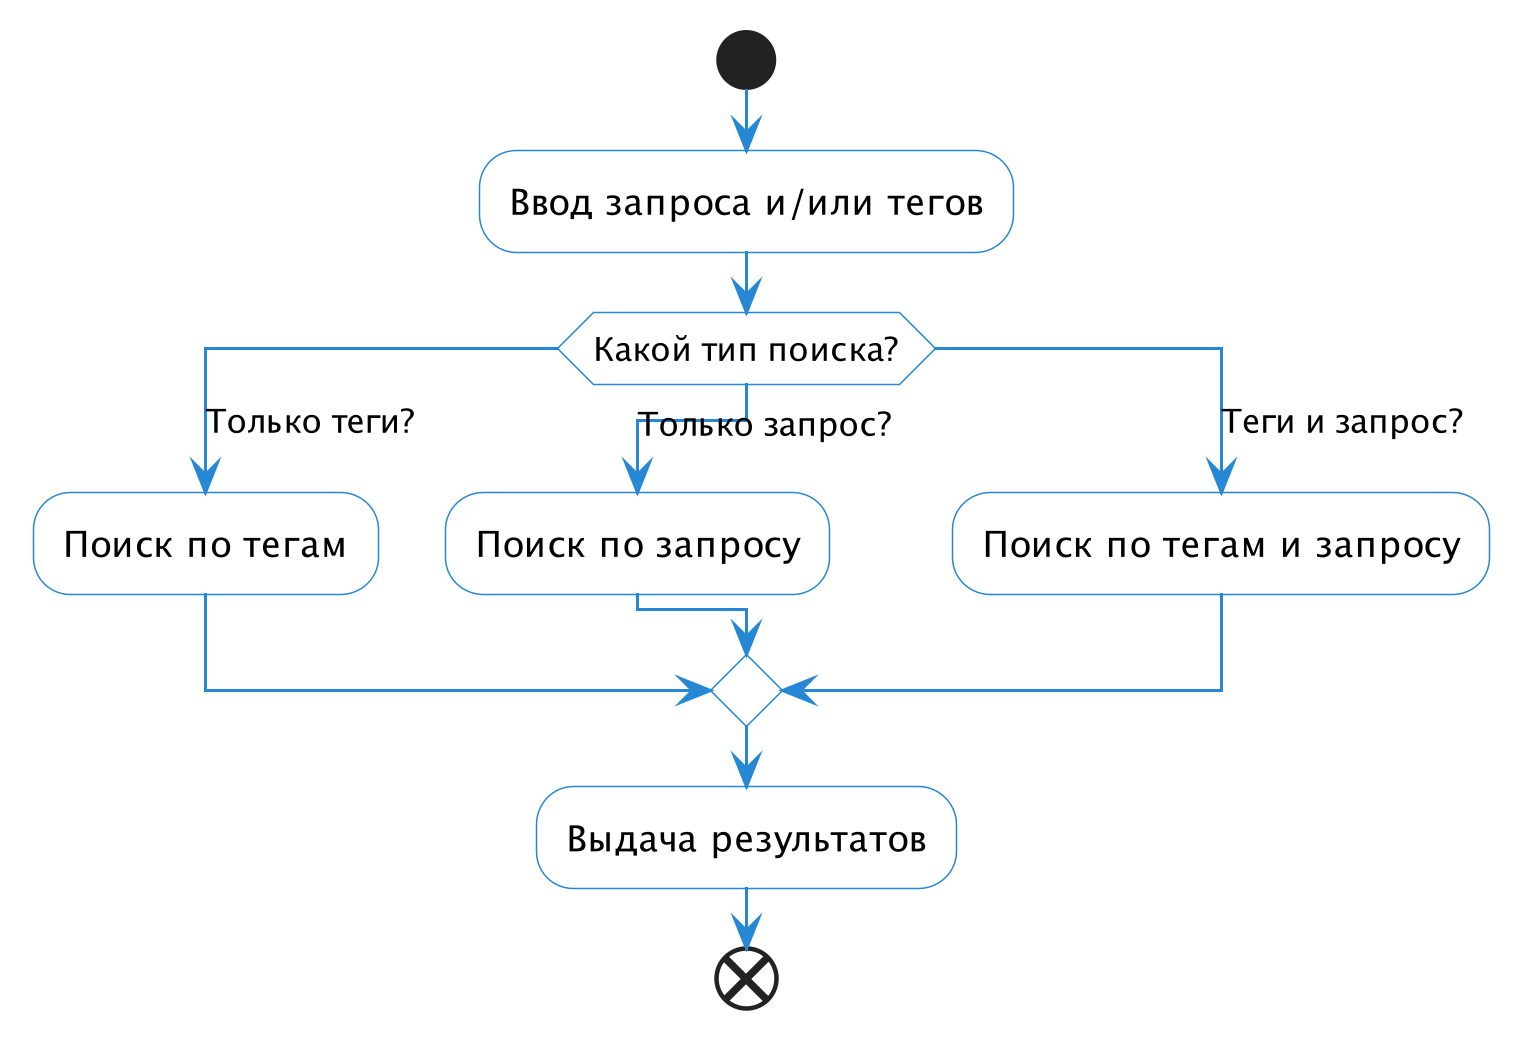
\includegraphics[width=0.8\textwidth]{images/search.png}
    \caption{Диаграмма поиска товаров}
    \label{fig:search}
\end{figure}

Как говорилось ранее, наша площадка рассчитана на креативные товары, а потому какие-то конкретные категории выделить очень сложно. Именно поэтому вместо категорий на нашей площадке используются теги. Эти теги похожи на привычные теги из социальных сетей: добавляет их продавец, а нужны они для упрощения поиска. Кроме тегов, также можно использовать обычный текстовый поиск.

\subsection{Взаимодействие с товарами}

Основной функционал нашей площадки завязан на товарах. В этом разделе будет рассмотрены следующие возможности по взаимодействию с товарами:
\begin{itemize}
    \item выставление товара на продажу;
    \item изменение товара;
    \item добавление товара в избранное.
\end{itemize}

\subsubsection*{Выставление товара на продажу}

Рассмотрим подробнее процесс выставления товару на продажу. Для этого зарегистрированный пользователь с подпиской должен заполнить форму, в которой он должен добавить следующую информацию о товаре:
\begin{itemize}
    \item название товара;
    \item стоимость;
    \item описание;
    \item изображения товара.
\end{itemize}
Кроме того, пользователь может добавить свои контактные данные в виде телефона и адреса электронной почты. Схема создания товара отражена на рисунке \ref{fig:add_item}.

\begin{figure}[H]
    \centering
    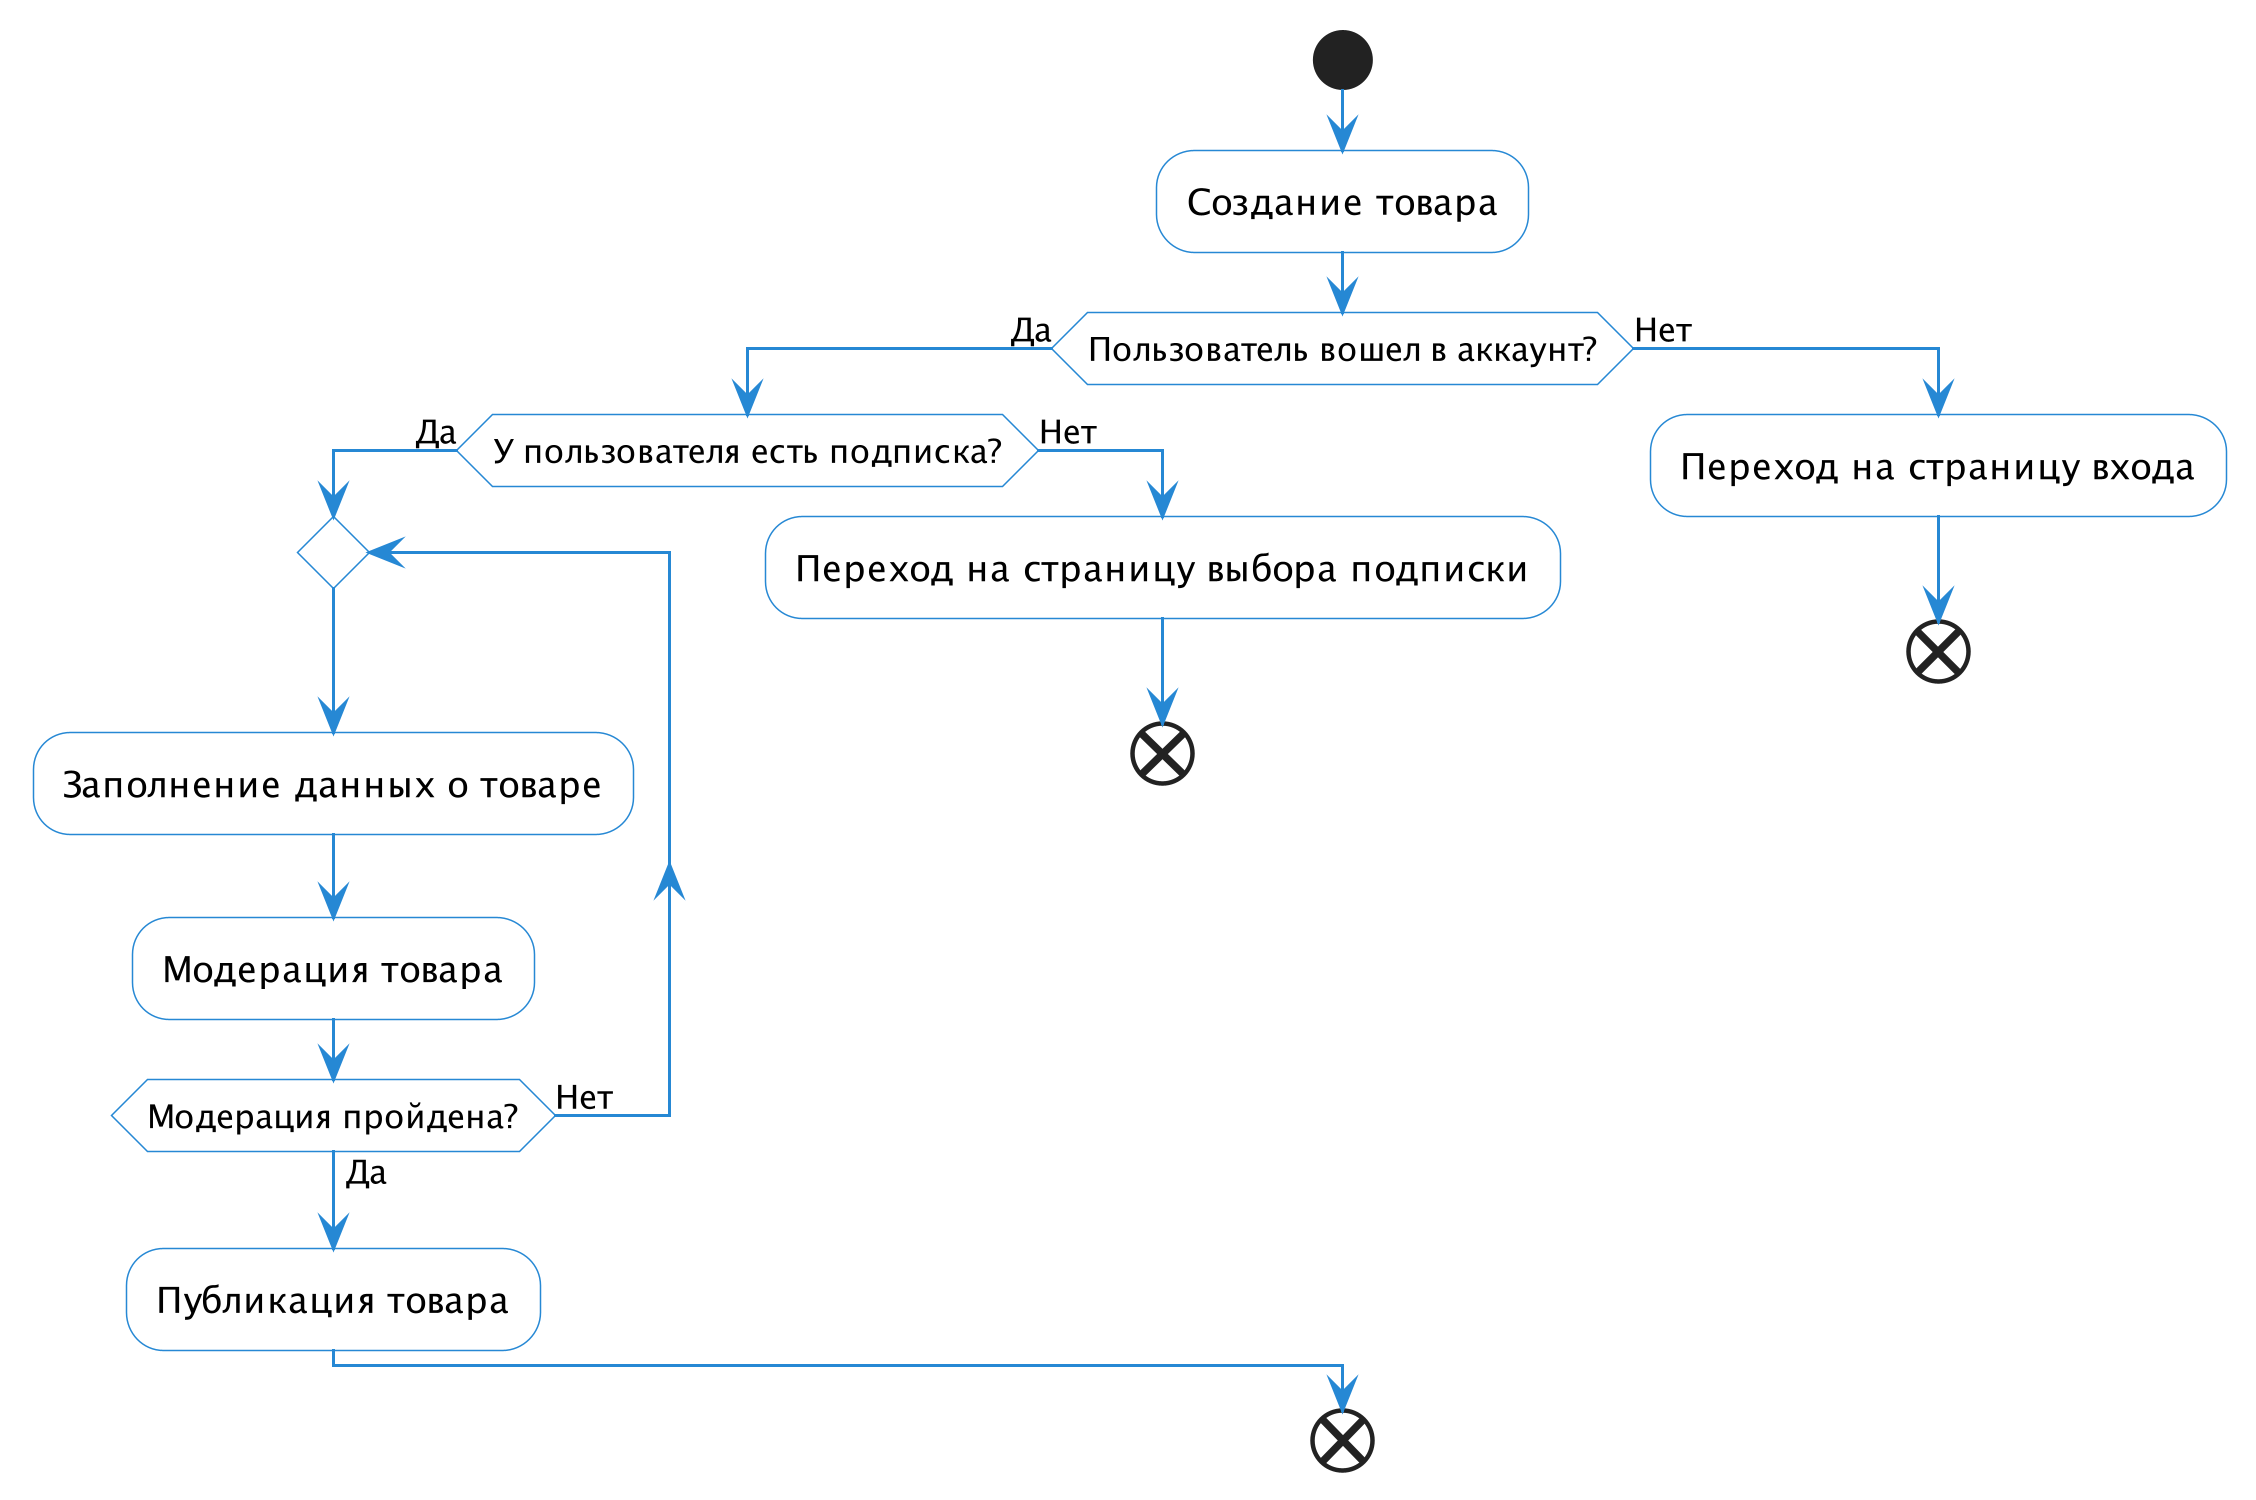
\includegraphics[width=\textwidth]{images/add_item.png}
    \caption{Диаграмма добавления товара на продажу}
    \label{fig:add_item}
\end{figure}

После заполнения формы товар отправляется на модерацию. На модерации товар проверятся по следующим критериям:
\begin{itemize}
    \item \textit{уникальность}: товар не должен быть самым обычным, доступным на каждом углу;
    \item \textit{приемлемое качество}: товар не должен выглядеть как мусор;
    \item \textit{креативность}: товар должен быть интересным, цепляющимся за глаз.
\end{itemize}
Таким образом, модерацию не смогут пройти следующие вещи:
\begin{itemize}
    \item товары широкого потребления;
    \item товары низкого качества;
    \item товары, не содержащие креативной идеи.
\end{itemize}

\subsubsection*{Изменение товара}

После выставления товара на продажу, через некоторое время может появиться необходимость в изменении состояния товара. Так, пользователю доступны следующие состояния товара:
\begin{itemize}
    \item доступен к покупке;
    \item нет в наличии;
    \item продан.
\end{itemize}
Схема изменения состояния товара изображена на рисунке \ref{fig:change_item}.

\begin{figure}[H]
    \centering
    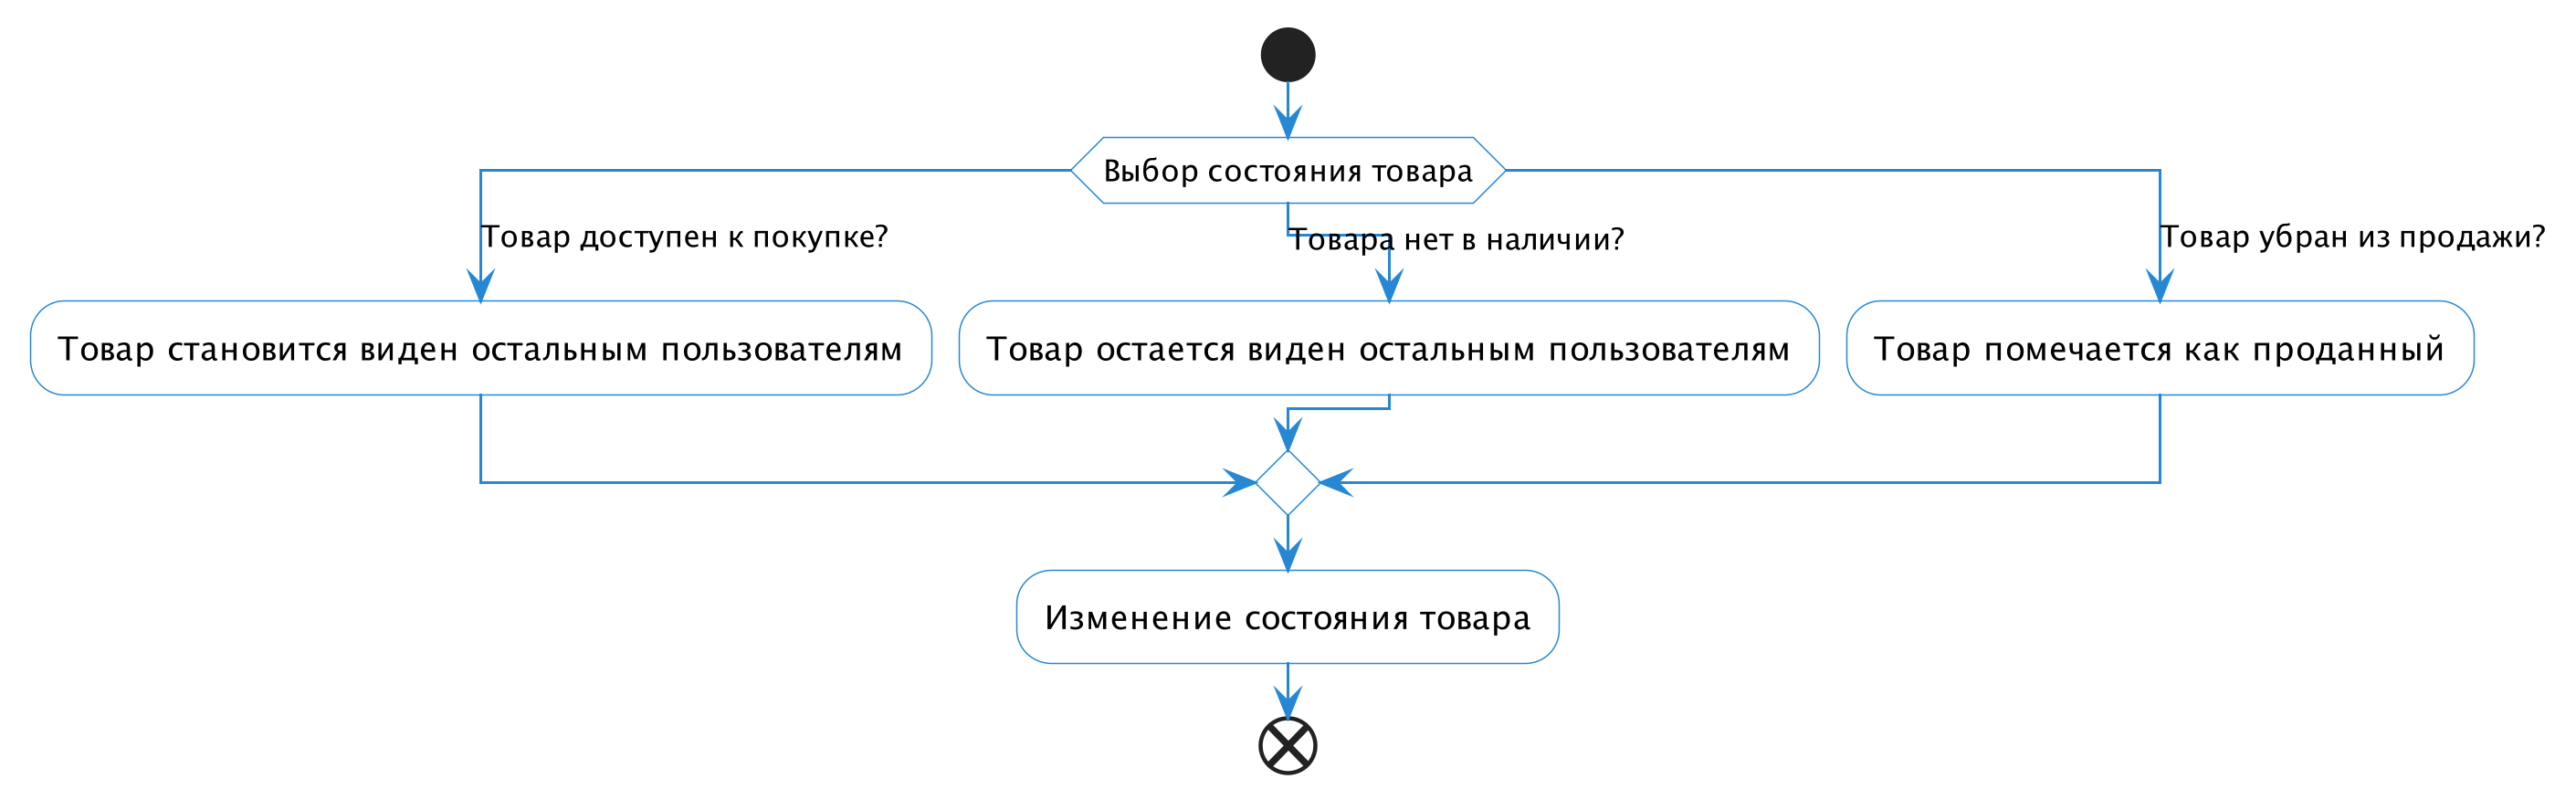
\includegraphics[width=\textwidth]{images/change_item.png}
    \caption{Диаграмма изменения состояния товара}
    \label{fig:change_item}
\end{figure}

В случае, когда товар помечается как доступный к покупке, товар становится виден всем пользователям площадки. При изменении состояния на нет в наличии, товар все еще остается виден пользователям. Однако, если пользователь пометит товар как проданный, то товар будет виден только продавцу. Остальные пользователи площадки не смогут найти его.

\subsubsection*{Добавление товара в избранное}

Чаще всего пользователи делают выбор из нескольких товаров. Поэтому было бы удобно, если можно было бы сохранить понравившиеся товары в отдельный список. Эту функцию реализует система избранных товаров. Пользователю достаточно всего лишь добавить товар в избранное, чтобы не потерять его. Диаграмма добавления товара в избранное показана на рисунке \ref{fig:add_to_favourites}.

\begin{figure}[H]
    \centering
    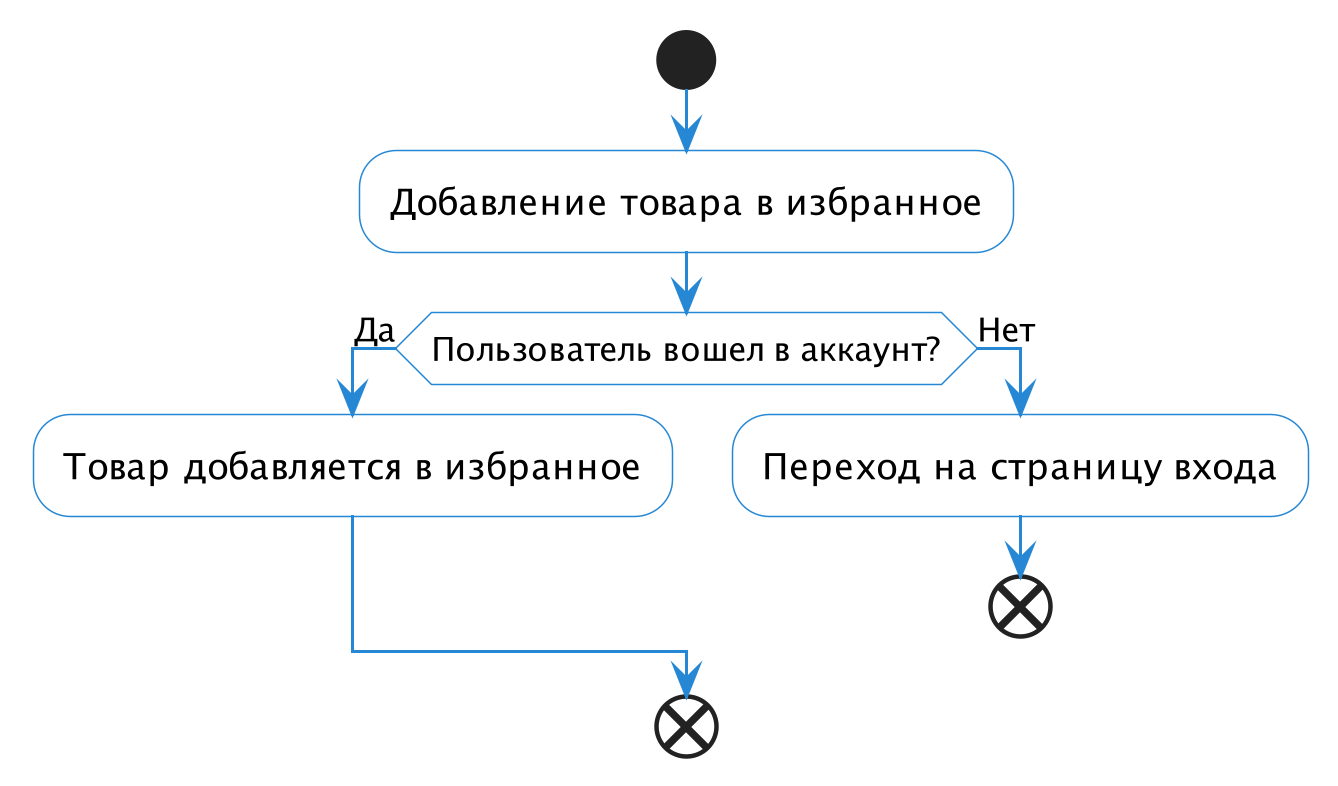
\includegraphics[width=0.7\textwidth]{images/add_to_favourites.png}
    \caption{Диаграмма добавления товара в избранное}
    \label{fig:add_to_favourites}
\end{figure}

Единственное условие -- пользователь должен быть авторизован. Мы требуем это, поскольку товары, добавленные в избранное, относятся к конкретному пользователю.

\subsection{Вход в аккаунт}

Теперь рассмотрим процесс входа в аккаунт. Как и всегда, вход в аккаунт делится на две составляющие: регистрацию и авторизацию. Схема входа в аккаунт показана на рисунке \ref{fig:login}.

\begin{figure}[H]
    \centering
    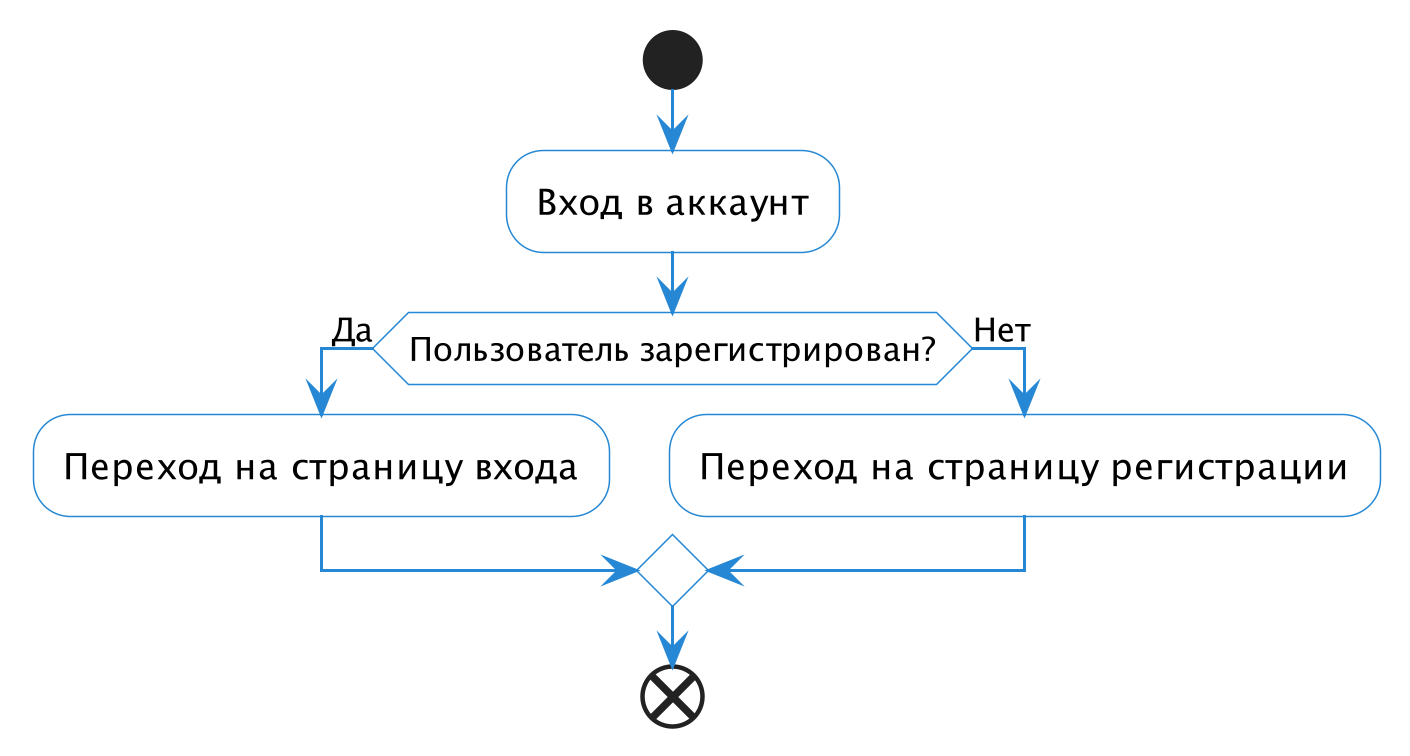
\includegraphics[width=0.7\textwidth]{images/login.png}
    \caption{Диаграмма входа в аккаунт}
    \label{fig:login}
\end{figure}

\subsubsection*{Регистрация}

При регистрации проверяется корректность введенных данных. Точнее, проверяются следующие критерии:
\begin{itemize}
    \item пользователя с данной электронной почтой не существует;
    \item пользователя с данным ником не существует;
    \item ник не содержит запрещенных слов;
    \item пароль состоит минимум из 8 символов.
\end{itemize}
После регистрации пользователь попадает на страницу авторизации. Схема создания аккаунта показан на рисунке \ref{fig:register}.

\begin{figure}[H]
    \centering
    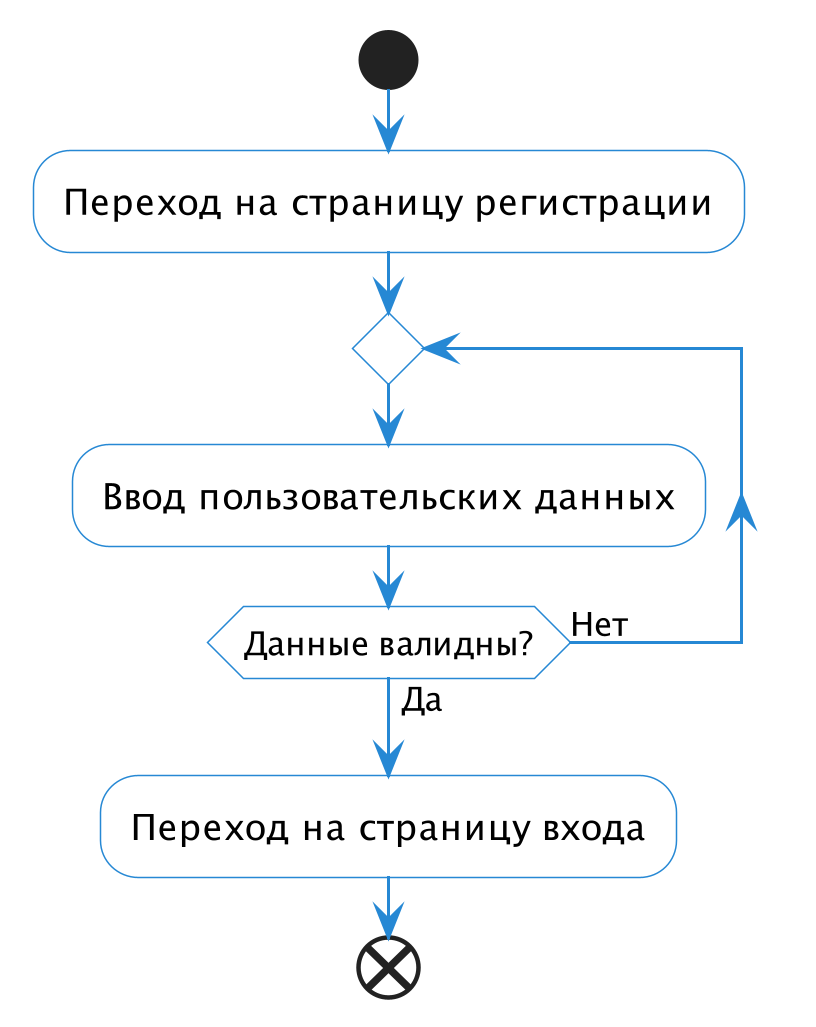
\includegraphics[height=0.4\textheight]{images/register.png}
    \caption{Диаграмма регистрации}
    \label{fig:register}
\end{figure}

\subsubsection*{Авторизация}

При авторизации сначала проверяется корректность введенных данных. После этого, проверяется, подтвержден ли текущий аккаунт. Аккаунт подтверждается с помощью перехода по ссылке, которая приходит на электронную почту. Если аккаунт подтвержден, то процесс авторизации завершен. Иначе, пользователь может потребовать выслать новую ссылку для подтверждения аккаунта. Процесс авторизации изображен на рисунке \ref{fig:auth}.

\begin{figure}[H]
    \centering
    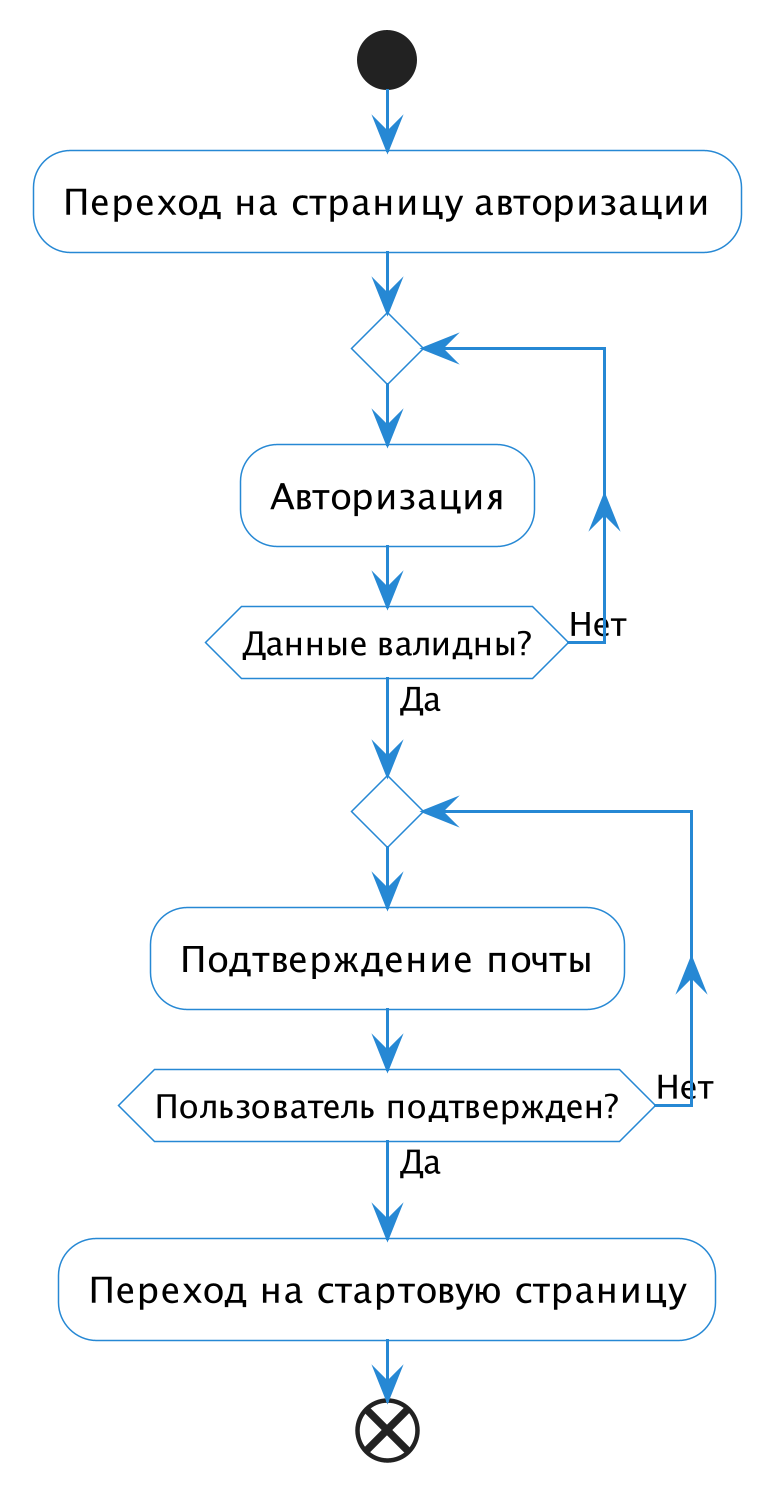
\includegraphics[height=0.5\textheight]{images/auth.png}
    \caption{Диаграмма авторизации}
    \label{fig:auth}
\end{figure}

\subsection{Приобретение подписки}

Для добавления товара на площадку необходимо выполнить как минимум два условия: быть авторизованным и иметь подписку на своем аккаунте. Схема добавления товара показана на рисунке \ref{fig:subscription}. Рассмотрим процесс приобретения подписки подробнее.

\begin{figure}[H]
    \centering
    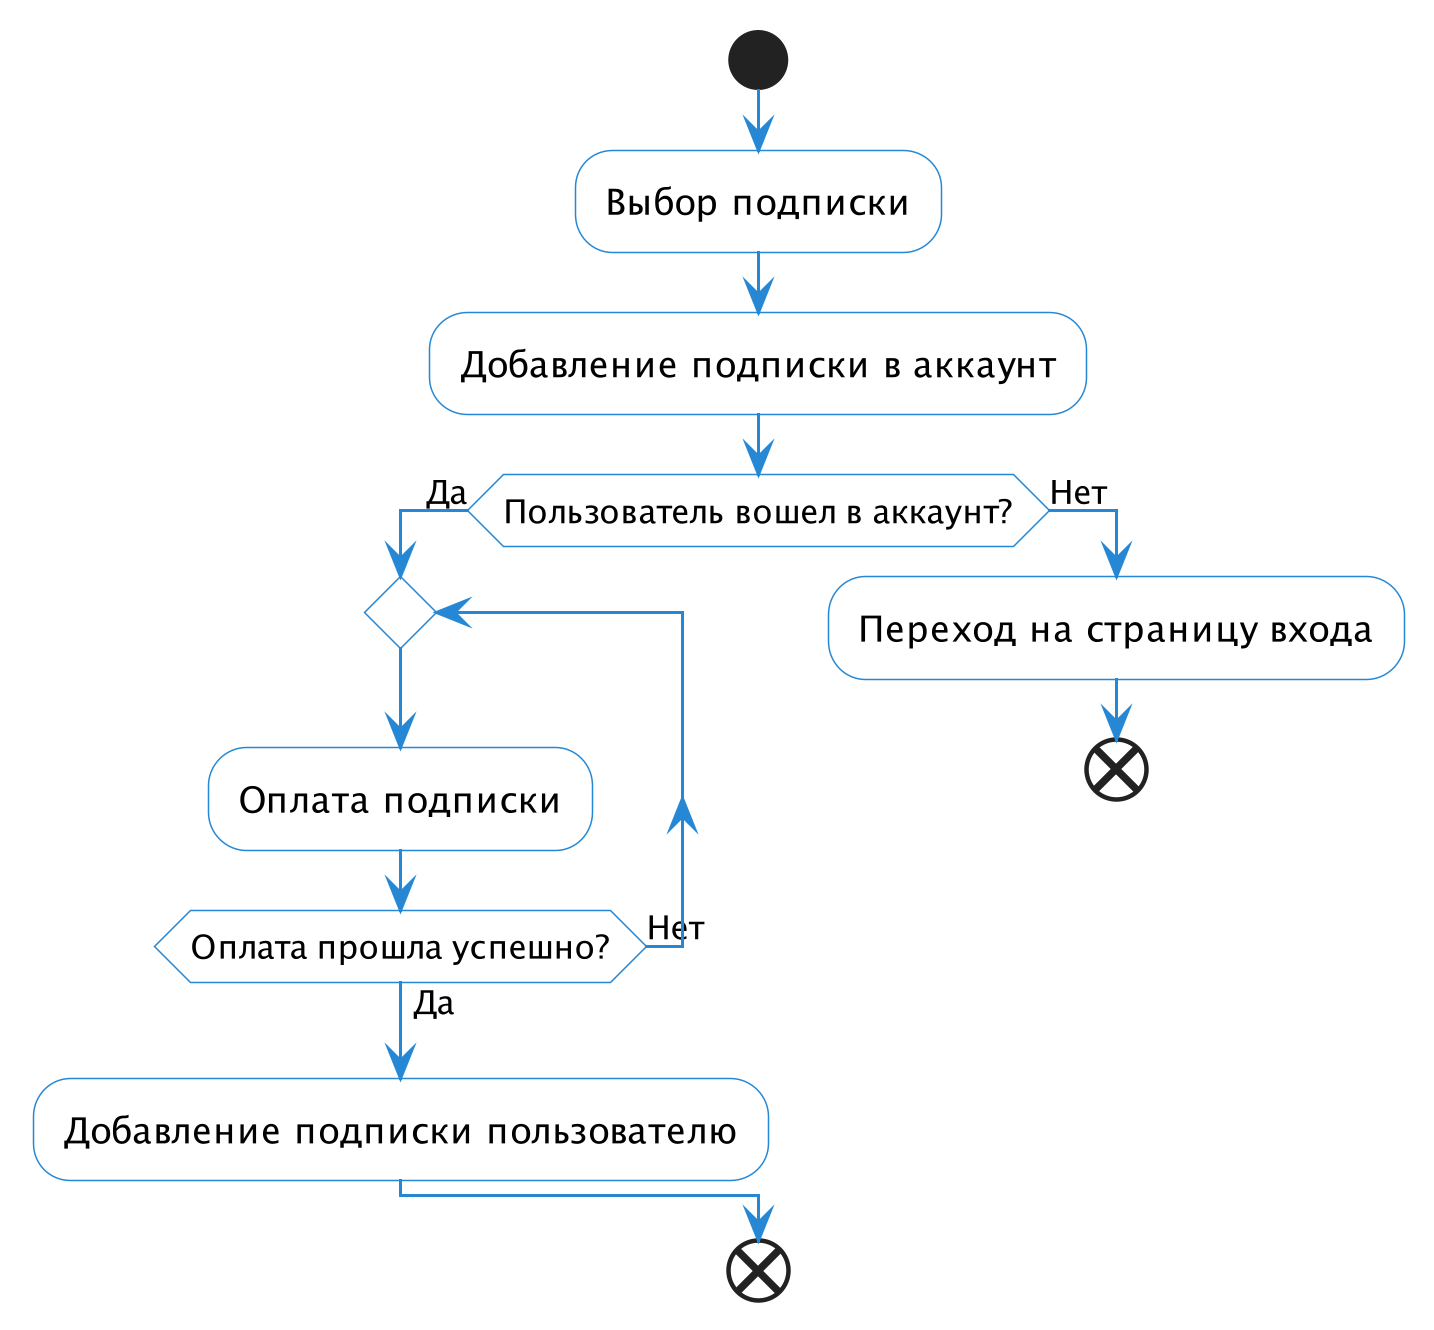
\includegraphics[width=0.65\textwidth]{images/subscription.png}
    \caption{Диаграмма добавления подписки}
    \label{fig:subscription}
\end{figure}

Прежде всего, пользователю необходимо определиться, какую подписку он собирается приобрести. В таблице \ref{tab:subscription_example} приведены примеры видов подписок.

\begin{center}
    \begin{longtable}{|>{\centering\arraybackslash}m{5cm}|>{\centering\arraybackslash}m{5cm}|>{\centering\arraybackslash}m{5.5cm}|}
        \caption{Примеры подписок}
        \label{tab:subscription_example}
        \\
        \hline
        \textbf{Название} & \textbf{Длительность} & \textbf{Стоимость} \\
        \hline
        Право имеющий     & 1 месяц               & 300 рублей         \\
        \hline
        Твоя роза         & 3 месяца              & 777 рублей         \\
        \hline
        Замена счастию    & 6 месяцев             & 1337 рублей        \\
        \hline
        Часть той силы    & 12 месяцев            & 2048 рублей        \\
        \hline
    \end{longtable}
\end{center}

После выбора подписки, пользователь должен оплатить ее. В случае успешного завершения оплаты, подписка добавляется на аккаунт пользователя.

\subsection{Добавление отзывов}

Пользователи могут добавлять отзывы на продавцов. В отличии от товаров, отзывы видны сразу после их добавления. Однако отзыв может быть удален, если не он не пройдет модерацию. Схема добавления отзывов отображена на рисунке \ref{fig:user_feedback}.

\begin{figure}[H]
    \centering
    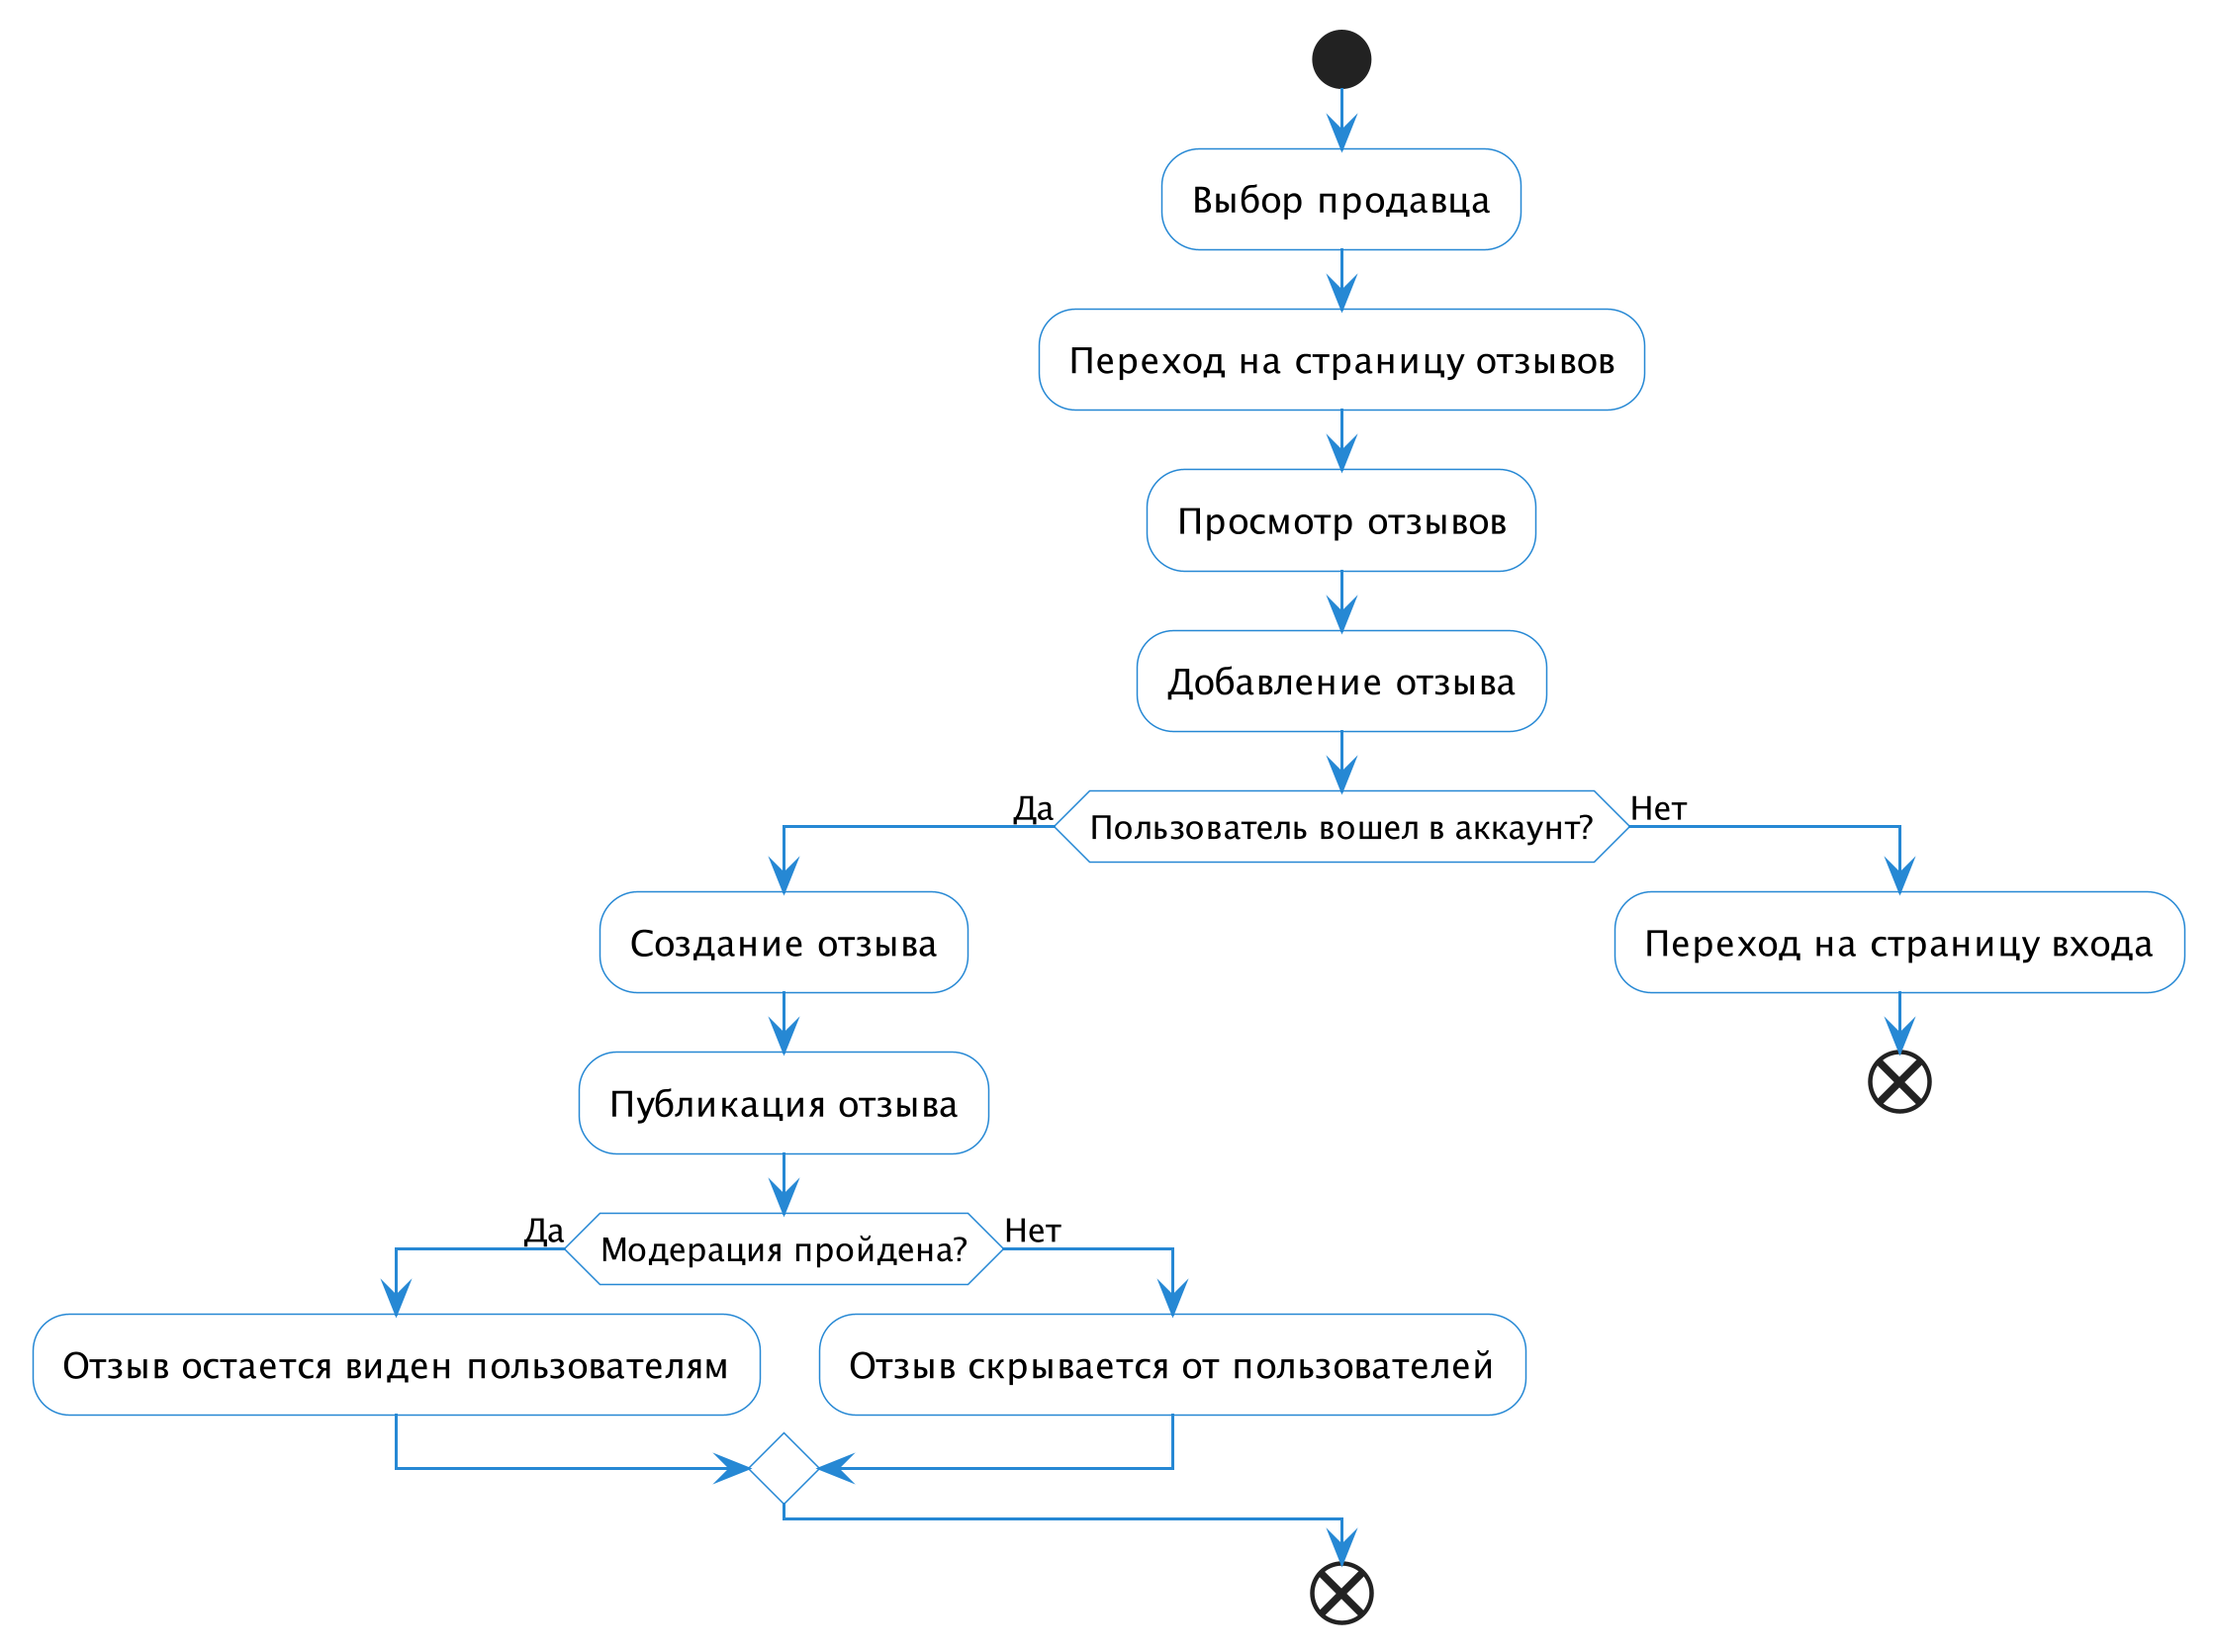
\includegraphics[width=\textwidth]{images/user_feedback.png}
    \caption{Диаграмма добавления отзыва к продавцу}
    \label{fig:user_feedback}
\end{figure}

\section{Проектирование базы данных}

На рисунках \ref{fig:uml-db} и \ref{fig:eer-db} представлены схемы получившейся в ходе разработки базы данных. В этом разделе мы подробно рассмотрим причины тех или иных решений.

\begin{figure}[H]
    \centering
    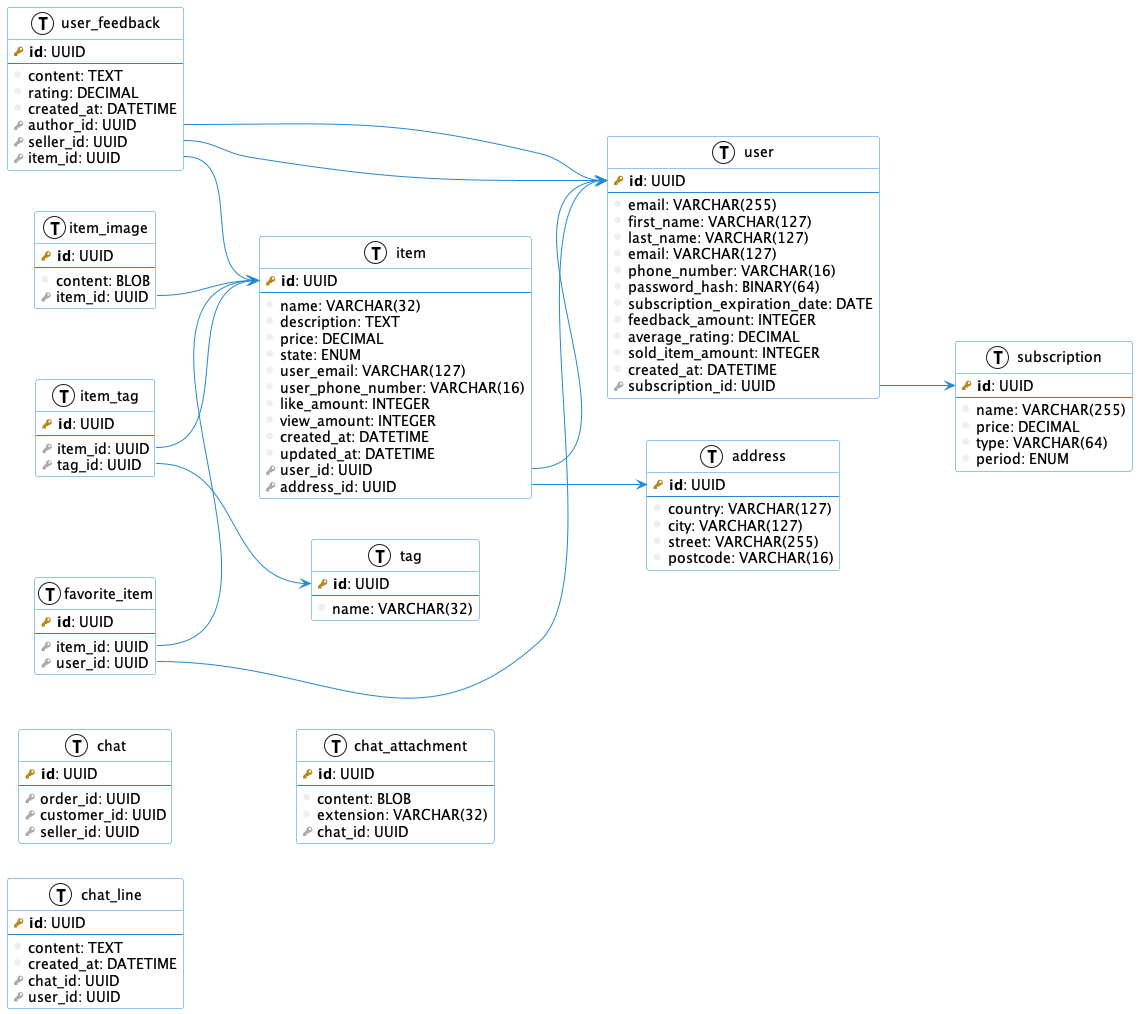
\includegraphics[width=\textwidth]{images/db.png}
    \caption{UML диаграмма базы данных}
    \label{fig:uml-db}
\end{figure}

\begin{figure}[H]
    \centering
    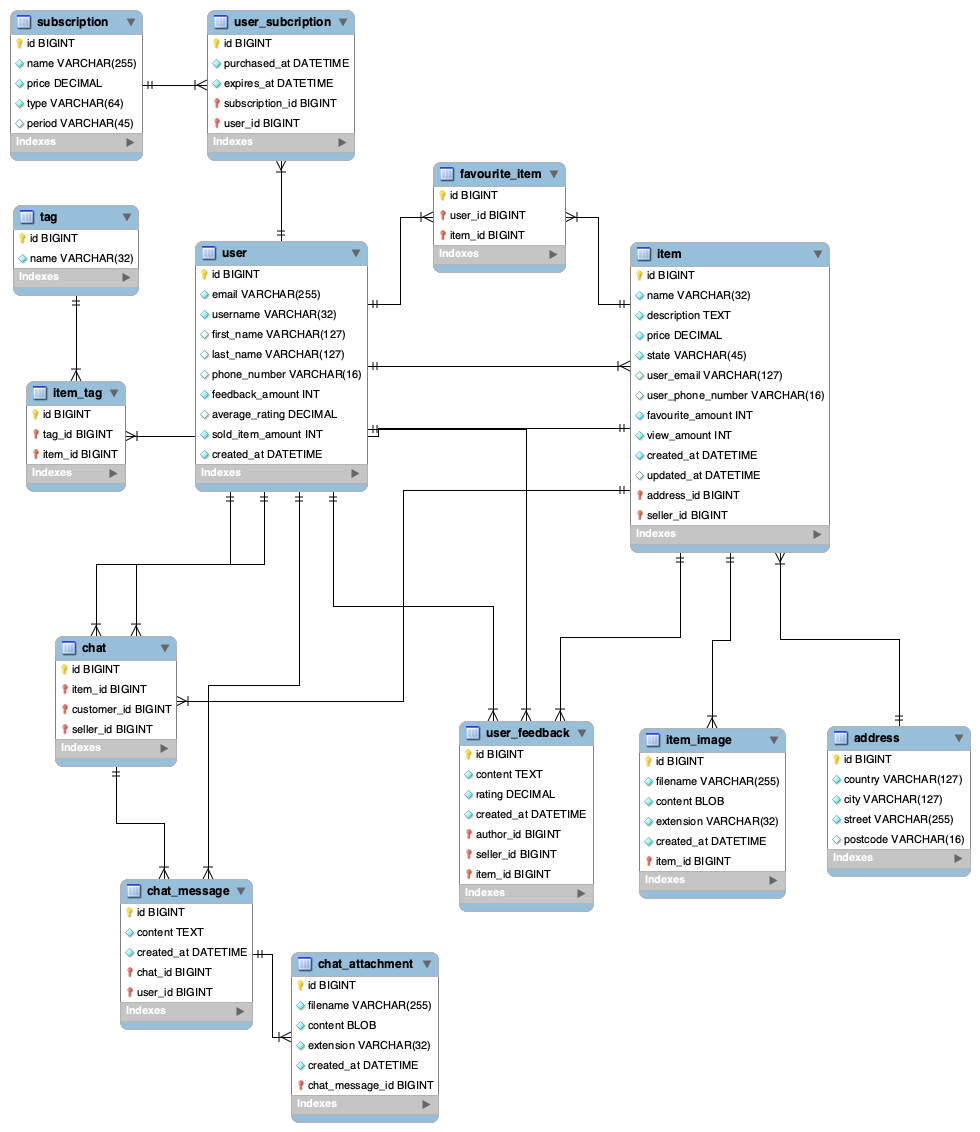
\includegraphics[width=\textwidth]{images/eer.png}
    \caption{EER диаграмма базы данных}
    \label{fig:eer-db}
\end{figure}

\subsection{Пользователи}

Для начала рассмотрим устройство пользователя в нашей системе. Прежде всего каждый пользователь должен иметь информацию об электронной почте, нике и пароле. Для безопасности пароль будем хранить в захешированном виде. Кроме того, пользователь также может указать информацию о своем имени и фамилии, номере телефона. Поскольку мы предполагаем наличие рейтинговой системы у каждого пользователя, нам также нужно хранить количество отзывов и их среднее значение. Также было решено хранить дату создания аккаунта и количество проданных товаров. Описание получившихся полей этой таблицы представлено в таблице \ref{tab:user}.

\begin{center}
    \begin{longtable}{|c|c|>{\centering\arraybackslash}m{8cm}|}
        \caption{Описание полей таблицы \texttt{user}}
        \label{tab:user}
        \\
        \hline
        \textbf{Название}           & \textbf{Тип}           & \textbf{Описание}                                                                     \\
        \hline
        \texttt{id}                 & \texttt{UUID}          & Идентификатор пользователя. Первичный ключ                                            \\
        \hline
        \texttt{email}              & \texttt{VARCHAR(255)}  & Почта пользователя. Обязательное и уникальное поле                                    \\
        \hline
        \texttt{username}           & \texttt{VARCHAR(32)}   & Ник пользователя. Обязательное и уникальное поле. Не менее 4 символов                 \\
        \hline
        \texttt{first\_name}        & \texttt{VARCHAR(127)}  & Имя пользователя                                                                      \\
        \hline
        \texttt{last\_name}         & \texttt{VARCHAR(127)}  & Фамилия пользователя                                                                  \\
        \hline
        \texttt{phone\_number}      & \texttt{VARCHAR(16)}   & Телефонный номер пользователя. Уникальное поле                                        \\
        \hline
        \texttt{password\_hash}     & \texttt{CHAR(16)}      & Хеш пароль пользователя (SHA-256). Обязательное поле                                  \\
        \hline
        \texttt{feedback\_amount}   & \texttt{INTEGER}       & Количество отзывов у пользователя как продавца. Значение по умолчанию -- \texttt{0}   \\
        \hline
        \texttt{average\_rating}    & \texttt{DECIMAL(3, 2)} & Средний рейтинг пользователя как продавца. Значение варьируется в интервале от 1 до 5 \\
        \hline
        \texttt{sold\_item\_amount} & \texttt{INTEGER}       & Количество проданных товаров. Значение по умолчанию -- \texttt{0}                     \\
        \hline
        \texttt{created\_at}        & \texttt{DATETIME}      & Дата создания аккаунта                                                                \\
        \hline
    \end{longtable}
\end{center}

Теперь рассмотрим подписочную систему. Прежде всего, у подписки должны быть определены названия, стоимость и время действия. Кроме того, в каждой подписке будем хранить ее тип. Это позволить гибко фильтровать подписки в зависимости от ситуации (например, нам нужно ввести подписки для Нового года, при этом должна быть возможность отображать как старую, так и новую цену). Описание получившихся полей этой таблицы представлено в таблице \ref{tab:subscription}.

\begin{center}
    \begin{longtable}{|c|c|>{\centering\arraybackslash}m{9.8cm}|}
        \caption{Описание полей таблицы \texttt{subscription}}
        \label{tab:subscription}
        \\
        \hline
        \textbf{Название} & \textbf{Тип}           & \textbf{Описание}                                                                                                                               \\
        \hline
        \texttt{id}       & \texttt{UUID}          & Идентификатор подписки. Первичный ключ                                                                                                          \\
        \hline
        \texttt{name}     & \texttt{VARCHAR(255)}  & Название подписки. Обязательно поле                                                                                                             \\
        \hline
        \texttt{price}    & \texttt{DECIMAL(15,4)} & Стоимость подписки. Обязательное поле                                                                                                           \\
        \hline
        \texttt{type}     & \texttt{VARCHAR(64)}   & Тип подписки. Обязательное поле                                                                                                                 \\
        \hline
        \texttt{period}   & \texttt{ENUM}          & Время действия подписки. В \texttt{ENUM} содержатся следующие значения: \texttt{MONTH}, \texttt{THREE MONTH}, \texttt{HALF YEAR}, \texttt{YEAR} \\
        \hline
    \end{longtable}
\end{center}

Теперь рассмотрим то, как связаны пользователи и подписки. Несмотря на то, что в конкретный момент времени пользователь может иметь только одну активную подписку, нам необходимо хранить не только текущую, но и все предыдущие подписки. Это позволит, при необходимости, ввести систему скидок, которая будет зависеть от количества предыдущих купленных подписок.

Каждая подписка пользователя должна содержать информацию о начале и об окончании срока подписки, а также идентификаторы пользователя и конкретной подписки. Исходя из этого описания, получаем, что мы имеем связь многие ко многим, поскольку один пользователь мог использовать несколько разных подписок за все время, равно как и одна подписка может использоваться у нескольких пользователей сразу. Описание получившихся полей этой таблицы представлено в таблице \ref{tab:user_subscription}.

\begin{center}
    \begin{longtable}{|c|c|>{\centering\arraybackslash}m{9.2cm}|}
        \caption{Описание полей таблицы \texttt{user\_subscription}}
        \label{tab:user_subscription}
        \\
        \hline
        \textbf{Название}         & \textbf{Тип}      & \textbf{Описание}                                                                      \\
        \hline
        \texttt{id}               & \texttt{UUID}     & Идентификатор подписки пользователя. Первичный ключ                                    \\
        \hline
        \texttt{purchased\_at}    & \texttt{DATETIME} & Дата приобретения подписки. Обязательное поле                                          \\
        \hline
        \texttt{expires\_at}      & \texttt{DATETIME} & Дата истечения подписки. Обязательное поле                                             \\
        \hline
        \texttt{user\_id}         & \texttt{UUID}     & Идентификатор пользователя. Внешний ключ на таблицу \texttt{user} поле \texttt{id}     \\
        \hline
        \texttt{subscription\_id} & \texttt{UUID}     & Идентификатор подписки. Внешний ключ на таблицу \texttt{subscription} поле \texttt{id} \\
        \hline
    \end{longtable}
\end{center}

Рассмотрим устройство отзывов на продавцов. Каждый отзыв должен включать в себя свое содержимое, оценку продавца и дату создания отзыва. Кроме этого, поскольку отзывы завязаны на определенный товар, продавца и покупателя, мы должны хранить идентификаторы этих сущностей. Описание получившихся полей этой таблицы представлено в таблице \ref{tab:user_feedback}.

\begin{center}
    \begin{longtable}{|c|c|>{\centering\arraybackslash}m{10.5cm}|}
        \caption{Описание полей таблицы \texttt{user\_feedback}}
        \label{tab:user_feedback}
        \\
        \hline
        \textbf{Название}    & \textbf{Тип}          & \textbf{Описание}                                                                                             \\
        \hline
        \texttt{id}          & \texttt{UUID}         & Идентификатор отзыва. Первичный ключ                                                                          \\
        \hline
        \texttt{content}     & \texttt{TEXT}         & Текстовое содержание отзыва. Обязательное поле                                                                \\
        \hline
        \texttt{rating}      & \texttt{DECIMAL(3,2)} & Оценка, которую поставил пользователь продавцу. Обязательное поле. Значение варьируется в интервале от 1 до 5 \\
        \hline
        \texttt{created\_at} & \texttt{DATETIME}     & Дата создания отзыва. Обязательное поле                                                                       \\
        \hline
        \texttt{author\_id}  & \texttt{UUID}         & Идентификатор автора отзыва. Внешний ключ на таблицу \texttt{user} поле \texttt{id}                           \\
        \hline
        \texttt{seller\_id}  & \texttt{UUID}         & Идентификатор продавца. Внешний ключ на таблицу \texttt{user} поле \texttt{id}                                \\
        \hline
        \texttt{item\_id}    & \texttt{UUID}         & Идентификатор товара. Внешний ключ на таблицу \texttt{item} поле \texttt{id}                                  \\
        \hline
    \end{longtable}
\end{center}

Рассмотрим систему добавления товара в избранное. Для реализации этой системы нам необходимо хранить идентификатор пользователя, добавившего товар, и идентификатор самого товара. Из этого следует, что имеем связь многие ко многим, поскольку несколько товаров может быть добавлено в избранное одним пользователем. В то же время один товар может быть добавлен в избранное несколькими пользователями. Описание получившихся полей этой таблицы представлено в таблице \ref{tab:favourite_item}.

\begin{center}
    \begin{longtable}{|c|c|>{\centering\arraybackslash}m{11.9cm}|}
        \caption{Описание полей таблицы \texttt{favourite\_item}}
        \label{tab:favourite_item}
        \\
        \hline
        \textbf{Название} & \textbf{Тип}  & \textbf{Описание}                                                                  \\
        \hline
        \texttt{id}       & \texttt{UUID} & Идентификатор понравившегося товара. Первичный ключ                                \\
        \hline
        \texttt{item\_id} & \texttt{UUID} & Идентификатор товара. Внешний ключ на таблицу \texttt{item} поле \texttt{id}       \\
        \hline
        \texttt{user\_id} & \texttt{UUID} & Идентификатор пользователя. Внешний ключ на таблицу \texttt{user} поле \texttt{id} \\
        \hline
    \end{longtable}
\end{center}

\subsection{Товары}

Рассмотрим устройство товаров. Каждый товар должен включать название, описание и стоимость. Кроме того, он дополнительно может включат в себя информацию о электронной почте и телефонном номере продавца. Также у каждого товара есть состояние (например, товар находится на модерации). Также, поскольку у пользователей есть возможность добавлять товары в избранное, было решено добавить счетчик людей, добавивших в избранное. Чтобы лучше продвигать тот или иной товар, было решено также хранить количество просмотров товара. Кроме того, мы решили добавить дату создания и дату изменения товара. В добавок ко всему вышеперечисленному, нам необходимо хранить идентификатор продавца. Также было решено у каждого объявления хранить адрес, чтобы ранжировать объявления по городам.

Исходя из вышеперечисленной информации, мы получаем связь один ко многим. Все потому, что у товара может быть только один продавец и один адрес. В это же время один и тот же адрес может быть у нескольких товаров, равно как и продавец может предлагать несколько товаров. Описание получившихся полей этой таблицы представлено в таблице \ref{tab:item}.

\begin{center}
    \begin{longtable}{|c|c|>{\centering\arraybackslash}m{7.5cm}|}
        \caption{Описание полей таблицы \texttt{item}}
        \label{tab:item}
        \\
        \hline
        \textbf{Название}            & \textbf{Тип}           & \textbf{Описание}                                                                                                                                                                     \\
        \hline
        \texttt{id}                  & \texttt{UUID}          & Идентификатор товара. Первичный ключ                                                                                                                                                  \\
        \hline
        \texttt{name}                & \texttt{VARCHAR(32)}   & Название товара. Обязательное поле                                                                                                                                                    \\
        \hline
        \texttt{description}         & \texttt{TEXT}          & Описание товара. Обязательное поле                                                                                                                                                    \\
        \hline
        \texttt{price}               & \texttt{DECIMAL(15,4)} & Стоимость товара. Обязательное поле                                                                                                                                                   \\
        \hline
        \texttt{state}               & \texttt{ENUM}          & Состояние товара. Обязательное поле. В \texttt{ENUM} содержатся следующие значения: \texttt{ON MODERATION}, \texttt{IN STOCK}, \texttt{OUT OF STOCK}, \texttt{SOLD}, \texttt{REMOVED} \\
        \hline
        \texttt{user\_email}         & \texttt{VARCHAR(127)}  & Электронная почта пользователя                                                                                                                                                        \\
        \hline
        \texttt{user\_phone\_number} & \texttt{VARCHAR(16)}   & Телефонный номер пользователя                                                                                                                                                         \\
        \hline
        \texttt{favourite\_amount}   & \texttt{INTEGER}       & Количество пользователей, добавивших товар в избранное. Значение по умолчанию -- \texttt{0}                                                                                           \\
        \hline
        \texttt{view\_amount}        & \texttt{INTEGER}       & Количество просмотров товара. Значение по умолчанию -- \texttt{0}                                                                                                                     \\
        \hline
        \texttt{created\_at}         & \texttt{DATETIME}      & Дата создания товара. Обязательное поле                                                                                                                                               \\
        \hline
        \texttt{updated\_at}         & \texttt{DATETIME}      & Дата изменения товара                                                                                                                                                                 \\
        \hline
        \texttt{seller\_id}          & \texttt{UUID}          & Идентификатор продавца. Внешний ключ на таблицу \texttt{user} поле \texttt{id}                                                                                                        \\
        \hline
        \texttt{address\_id}         & \texttt{UUID}          & Адрес продажи товара. Внешний ключ на таблицу \texttt{address} поле \texttt{id}                                                                                                       \\
        \hline
    \end{longtable}
\end{center}

Рассмотрим систему картинок товара. К каждому товару может быть приложено несколько картинок. Каждая картинка должна включать в себя имя файла, содержимое и расширение. Кроме этого картинка привязана к определенному товару. Исходя из этого получаем связь один ко многим, поскольку картинка может относится только к одному товару. Однако в то же время у одного товара может быть несколько картинок. Описание получившихся полей этой таблицы представлено в таблице \ref{tab:item_image}.

\begin{center}
    \begin{longtable}{|c|c|>{\centering\arraybackslash}m{10.5cm}|}
        \caption{Описание полей таблицы \texttt{item\_image}}
        \label{tab:item_image}
        \\
        \hline
        \textbf{Название}    & \textbf{Тип}          & \textbf{Описание}                                                            \\
        \hline
        \texttt{id}          & \texttt{UUID}         & Идентификатор изображения товара. Первичный ключ                             \\
        \hline
        \texttt{filename}    & \texttt{VARCHAR(255)} & Имя файла. Обязательное поле                                                 \\
        \hline
        \texttt{content}     & \texttt{BLOB}         & Двоичные данные файла. Обязательное поле                                     \\
        \hline
        \texttt{extension}   & \texttt{VARCHAR(32)}  & Расширение файла. Обязательное поле                                          \\
        \hline
        \texttt{created\_at} & \texttt{DATETIME}     & Дата создания изображения                                                    \\
        \hline
        \texttt{item\_id}    & \texttt{UUID}         & Идентификатор товара. Внешний ключ на таблицу \texttt{item} поле \texttt{id} \\
        \hline
    \end{longtable}
\end{center}

Рассмотрим систему тегов. Она довольно проста, поскольку тег должен включат в себя только имя. Описание получившихся полей этой таблицы представлено в таблице \ref{tab:tag}.

\begin{center}
    \begin{longtable}{|c|c|>{\centering\arraybackslash}m{10cm}|}
        \caption{Описание полей таблицы \texttt{tag}}
        \label{tab:tag}
        \\
        \hline
        \textbf{Название} & \textbf{Тип}         & \textbf{Описание}                  \\
        \hline
        \texttt{id}       & \texttt{UUID}        & Идентификатор тега. Первичный ключ \\
        \hline
        \texttt{name}     & \texttt{VARCHAR(32)} & Название тега. Обязательное поле   \\
        \hline
    \end{longtable}
\end{center}

Теперь рассмотрим применение тегов с товарами. Для этого необходимо хранить идентификатор товара, к которому прикреплен тег, а также идентификатор самого тега. Значит, мы имеем дело с связью многие ко многим, поскольку один товар может иметь несколько тегов, а один тег может относиться к нескольким товарам. Описание получившихся полей этой таблицы представлено в таблице \ref{tab:item_tag}.

\begin{center}
    \begin{longtable}{|c|c|>{\centering\arraybackslash}m{11.9cm}|}
        \caption{Описание полей таблицы \texttt{item\_tag}}
        \label{tab:item_tag}
        \\
        \hline
        \textbf{Название} & \textbf{Тип}  & \textbf{Описание}                                                            \\
        \hline
        \texttt{id}       & \texttt{UUID} & Идентификатор тега товара. Первичный ключ                                    \\
        \hline
        \texttt{item\_id} & \texttt{UUID} & Идентификатор товара. Внешний ключ на таблицу \texttt{item} поле \texttt{id} \\
        \hline
        \texttt{tag\_id}  & \texttt{UUID} & Идентификатор тега. Внешний ключ на таблицу \texttt{tag} поле \texttt{id}    \\
        \hline
    \end{longtable}
\end{center}

Рассмотрим адрес, используемый в описании товара. Каждый адрес обязательно должен включать в себя информацию о стране, городе и улице. Кроме этой информации, адрес может включать в себя почтовый индекс. Описание получившихся полей этой таблицы представлено в таблице \ref{tab:address}.

\begin{center}
    \begin{longtable}{|c|c|>{\centering\arraybackslash}m{9.9cm}|}
        \caption{Описание полей таблицы \texttt{address}}
        \label{tab:address}
        \\
        \hline
        \textbf{Название} & \textbf{Тип}          & \textbf{Описание}                    \\
        \hline
        \texttt{id}       & \texttt{UUID}         & Идентификатор адреса. Первичный ключ \\
        \hline
        \texttt{country}  & \texttt{VARCHAR(127)} & Название страны. Обязательное поле   \\
        \hline
        \texttt{city}     & \texttt{VARCHAR(127)} & Название города. Обязательное поле   \\
        \hline
        \texttt{street}   & \texttt{VARCHAR(255)} & Название улицы. Обязательное поле    \\
        \hline
        \texttt{postcode} & \texttt{VARCHAR(16)}  & Почтовый индекс                      \\
        \hline
    \end{longtable}
\end{center}

\subsection{Чат между покупателем и продавцом}

Перед покупкой товара у пользователя может появиться потребность пообщаться с продавцом. Например, покупатель захотел разузнать о товаре поподробнее или, например, пользователь готов купить товар. Для этого покупателю необходимо как-нибудь связаться с продавцом. Наша площадка предлагает несколько путей для решения этой проблемы.

Как было показано ранее, у каждого товара обязательно есть описание. Кроме того, к описанию можно добавить электронную почту и телефонный номер продавца. Таким образом, с помощью каких-либо контактных данных в описании товара, электронной почты или телефона покупатель может связаться с продавцом для уточнения своих вопросов.

Однако это не единственный способ связи покупателя с продавцом. Наша площадка предоставляет минимально необходимый функционал для общения покупателей и продавцов. Для каждого товара между покупателем и продавцом создается чат, в котором можно отправлять как текстовые сообщения, так и различные файлы, в том числе и картинки.

Исходя из вышеописанного функционала, можно выделить три сущности: чат, сообщения и вложения. Рассмотрим каждый из них поподробнее.

Начнем с таблицы чатов. Как было сказано ранее, чаты формируются отдельно для покупателя и продавца для каждого товара. Значит, нам нужно хранить идентификаторы покупателя и продавца, а также идентификатор товара.

Таким образом, мы получаем связь один к многим, поскольку конкретный чат может быть только между определенными пользователями. В то же время одни и те же покупатель и продавец могут переписываться на счет разных товаров. При этом, один продавец может иметь чат с несколькими клиентами для одного товара, а клиент может переписываться с несколькими продавцами на счет нескольких товаров сразу. Описание получившихся полей этой таблицы представлено в таблице \ref{tab:chat}.

\begin{center}
    \begin{longtable}{|c|c|>{\centering\arraybackslash}m{11.2cm}|}
        \caption{Описание полей таблицы \texttt{chat}}
        \label{tab:chat}
        \\
        \hline
        \textbf{Название}     & \textbf{Тип}  & \textbf{Описание}                                                                \\
        \hline
        \texttt{id}           & \texttt{UUID} & Идентификатор чата. Первичный ключ                                               \\
        \hline
        \texttt{item\_id}     & \texttt{UUID} & Идентификатор товара. Внешний ключ на таблицу \texttt{item} поле \texttt{id}     \\
        \hline
        \texttt{customer\_id} & \texttt{UUID} & Идентификатор покупателя. Внешний ключ на таблицу \texttt{user} поле \texttt{id} \\
        \hline
        \texttt{seller\_id}   & \texttt{UUID} & Идентификатор продавца. Внешний ключ на таблицу \texttt{user} поле \texttt{id}   \\
        \hline
    \end{longtable}
\end{center}

Теперь рассмотрим таблицу, отвечающую за хранение конкретного сообщения. Прежде всего каждое сообщение отправляется определенным пользователем, поэтому нам необходимо хранить идентификатор автора сообщения. Кроме того, каждое сообщение привязано к какому-то чату, значит, мы также должны хранить идентификатор чата. Кроме идентификаторов, также необходимо хранить содержимое сообщение и дату создания сообщения.

Исходя из описания, мы получаем связь один ко многим, поскольку определенное сообщение может быть отправлено только одним пользователем в определенном чате. В то же время, пользователь может отправлять несколько сообщений в разных чатах. Описание получившихся полей этой таблицы представлено в таблице \ref{tab:chat_message}.

\begin{center}
    \begin{longtable}{|c|c|>{\centering\arraybackslash}m{10.6cm}|}
        \caption{Описание полей таблицы \texttt{chat\_message}}
        \label{tab:chat_message}
        \\
        \hline
        \textbf{Название}    & \textbf{Тип}      & \textbf{Описание}                                                                      \\
        \hline
        \texttt{id}          & \texttt{UUID}     & Идентификатор сообщения. Первичный ключ                                                \\
        \hline
        \texttt{content}     & \texttt{TEXT}     & Содержание сообщения. Обязательное поле                                                \\
        \hline
        \texttt{created\_at} & \texttt{DATETIME} & Дата создания сообщения. Обязательное поле                                             \\
        \hline
        \texttt{chat\_id}    & \texttt{UUID}     & Идентификатор чата. Внешний ключ на таблицу \texttt{chat} поле \texttt{id}             \\
        \hline
        \texttt{user\_id}    & \texttt{UUID}     & Идентификатор автора сообщения. Внешний ключ на таблицу \texttt{user} поле \texttt{id} \\
        \hline
    \end{longtable}
\end{center}

Рассмотрим таблицу, которая будет хранить в себе содержимое вложения. В первую очередь нам необходимо хранить идентификатор сообщения, к которому относится это вложение. Кроме него, мы также будем хранить имя приложенного файла, его содержимое и расширение этого файла. Также будем хранить дату создания этого вложения.

В этот раз мы также получили связь один ко многим, потому что одно сообщение может включать в себя несколько вложений, однако одно и то же вложение может относиться только к одному сообщению. Описание получившихся полей этой таблицы представлено в таблице \ref{tab:chat_attachment}.

\begin{center}
    \begin{longtable}{|c|c|>{\centering\arraybackslash}m{8.2cm}|}
        \caption{Описание полей таблицы \texttt{chat\_attachment}}
        \label{tab:chat_attachment}
        \\
        \hline
        \textbf{Название}          & \textbf{Тип}          & \textbf{Описание}                                                                        \\
        \hline
        \texttt{id}                & \texttt{UUID}         & Идентификатор вложения. Первичный ключ                                                   \\
        \hline
        \texttt{filename}          & \texttt{VARCHAR(255)} & Имя файла. Обязательное поле                                                             \\
        \hline
        \texttt{content}           & \texttt{BLOB}         & Двоичные данные файла. Обязательное поле                                                 \\
        \hline
        \texttt{extension}         & \texttt{VARCHAR(32)}  & Расширение файла. Обязательное поле                                                      \\
        \hline
        \texttt{created\_at}       & \texttt{DATETIME}     & Дата загрузки файла. Обязательное поле                                                   \\
        \hline
        \texttt{chat\_message\_id} & \texttt{UUID}         & Идентификатор сообщения. Внешний ключ на таблицу \texttt{chat\_message} поле \texttt{id} \\
        \hline
    \end{longtable}
\end{center}

\section{Выводы}

В результате выполнения лабораторной работы была спроектирована база данных для интернет площадки для креативных людей. В процессе выполнения работы были выполнены все поставленные задачи. Получившаяся логическая схема базы данных удовлетворяет третьей нормальной форме.

Во время выполнения возникли некоторые сложности. В первую очередь, было очень сложно сбалансировать систему таким образом, чтобы товары пользователя были наравне с товарами других пользователей. При этом, проект нужно каким-то образом монетизировать. В качестве решения этой проблемы была выбрана подписочная система.

Еще одной сложностью стала проблема проектирования. Необходимо было спроектировать систему так, чтобы база данных была готова как к расширению, так и к более серьезным нагрузкам.

В итоге все проявившиеся проблемы удалось решить, как с точки зрения концепта, так и с точки зрения архитектуры базы данных.

\section{Список источников}

\begin{enumerate}
    \item MySQL Workbench [Электронный ресурс]. URL: \url{https://www.mysql.com/products/workbench/} (дата обращения: 05.12.2022).
    \item PlantUML [Электронный ресурс]. URL: \url{https://plantuml.com/en/} (дата обращения: 05.12.2022).
    \item Avito [Электронный ресурс]. URL: \url{https://www.avito.ru/} (дата обращения: 05.12.2022).
    \item Юла [Электронный ресурс]. URL: \url{https://youla.ru/} (дата обращения: 05.12.2022).
    \item Farpost [Электронный ресурс]. URL: \url{https://www.farpost.ru/} (дата обращения: 05.12.2022).
\end{enumerate}

\newpage

\section{Приложения}

\subsection*{\hfill Приложение 1}

\begin{center}
    \begin{longtable}{|c|>{\centering\arraybackslash}m{11.5cm}|}
        \caption{Состав команды}
        \label{tab:command}
        \\
        \hline
        \textbf{ФИ}      & \textbf{Роль}                                 \\
        \hline
        Швалов Даниил    & Проектирование архитектуры, создание диаграмм \\
        \hline
        Осыченко Арсений & Руководитель, генератор идей, аналитик        \\
        \hline
        Богданов Михаил  & Проектирование архитектуры, создание диаграмм \\
        \hline
        Ларичева Дарья   & Создатель отчета, генератор идей, аналитик    \\
        \hline
        Карагодин Максим & Проектирование архитектуры, создание диаграмм \\
        \hline
    \end{longtable}
\end{center}

\newpage

\subsection*{\hfill Приложение 2}

\subsubsection*{\centering Эссе (Швалов Д. А.)}

Базы данных окружают нас повсюду, практически во всех сферах жизни. Обычный обыватель может и не замечать, но спорить с этим бесполезно. Куда бы вы ни пришли, вы встретитесь с той или иной разновидностью баз данных.

Когда вы записываетесь в поликлинику, когда врач принимает вас, смотрит информацию о вас и ваших заболеваниях, тогда вы сталкиваетесь с базами данных. Когда вы приходите в столовую, кафе или ресторан, заказываете блюда, вы косвенно используете базы данных. Когда вы приходите в продуктовый магазин, набираете тележку товаров, взвешиваете некоторые из них, вы так или иначе взаимодействуете с базами данных. Список сфер, где используются базы данных можно продолжать до бесконечности: общественный транспорт, образовательные учреждения, все или почти все государственные учреждения, отели, места отдыха, системы видеонаблюдения, банковская сфера и так далее, и так далее.

Рассмотрим одну из сфер жизнедеятельности поподробнее. В сфере образования используется множество различных баз данных. Так, в основном, расписание пар или уроков хранится в базе данных. Оценки и баллы каждого ученика также хранятся в базе данных. Весь документооборот построен на базах данных. Запись на занятие и факультативы осуществляется через взаимодействие с базами данных. Даже бронирование помещений так или иначе использует базы данных.

Все это не спроста. Все потому, что базы данных позволяют в удобной форме просматривать, пополнять и изменять информацию, искать нужные сведения, делать необходимые выборки, осуществлять сортировку.

Рассмотрим пример использования этих операций. Пусть нам нужно приобрести билет на поезд. Чем нам могут помочь базы данных, кроме как хранением информации об отправлениях? Базы данных могут самостоятельно, опираясь на пользовательский запрос, отфильтровать и отсортировать нужную вам информацию. Таким образом, если нам нужны билеты из Санкт-Петербурга в Москву к определенной дате, в определенной вилке цен, отсортированный по стоимости билета, нам достаточно воспользоваться встроенными функциями базы данных. Она сможет справиться с этим запросом, и нам не придется прибегать к стороннему программному обеспечению. Именно эта универсальность, гибкость и удобство использования сделали современные базы данных такими популярными.

Однако такое обширное использование баз данных влечет за собой некоторые риски. Первый риск и самый очевидный — это несанкционированное чтение и слив персональных данных. Базы данных зачастую хранят множество личной информации. Именно она является лакомым кусочком для злоумышленников. Это, наверное, самый часто возникающий риск, с которым сталкивается каждый из нас.

Второй, не менее очевидный риск — потеря данных. При неправильном администрировании баз данных злоумышленники могут удалить всю базу данных, которая, скорее всего, содержит в себе ценную информацию за продолжительный срок. Потеря данных может привести к огромным убыткам как со стороны владельцев базы данных, так и со стороны ее пользователей.

Третий риск — несанкционированное измерение данных. Если злоумышленники получат доступ к несанкционированному изменению данных, они смогут манипулировать информацией, хранящейся в базе данных. Это, в свою очередь, в лучшем случае повлечет нарушение работы приложения, работающего с базой данных. В худшем случае это может привести к манипулированию пользователями, огромным убыткам компании и судебным искам.

Четвертый риск — распределений отказ в обслуживании или DDoS. Злоумышленник может не иметь прямого доступа к базе данных, однако это не означает полной защищенности базы данных. Так, злоумышленник может затруднить доступ других пользователей к вашей базе данных и попытаться перегрузить ее за счёт большого единовременного количества запросов с нескольких устройств. Хотя это звучит менее болезненно, чем все предыдущие риски, все равно этот способ атаки может принести огромные убытки для владельцев базы данных.

Базы данных стали неотъемлемой частью нашей повседневности. Они приносят удобство в нашу жизнь, делают ее проще. Однако они также имеют множество рисков, о которых стоит знать и к которым нужно быть готовым.

\newpage

\subsection*{\hfill Приложение 3}

\subsubsection*{\centering Кейс (Швалов Д. А.)}

Каждое мое утро начинается с будильника. Это первое приложение, которое я использую после пробуждения. Также это первое за день приложение, которое использует базы данных, поскольку приложение будильника должно хранить все будильники даже после выключения телефона. После пробуждения я открываю приложение my.itmo, чтобы посмотреть расписание. В нем также я встречаюсь с использованием баз данных, потому что расписания хранятся в базах данных. После этого, я сажусь завтракать. Обычно во время завтрака я смотрю видеоролики в приложении YouTube или КиноПоиск, которые хранят все видеофайлы в базах данных.

Позавтракав и собравшись, я отправляюсь в ВУЗ. Поскольку я живу достаточно далеко от ИТМО, мне приходится пользоваться метро. Чтобы попасть в метро, необходимо воспользоваться проездным. При прикладывании проездного терминал посылает данные о проездном на сервер. Сервер, в свою очередь, сверяет полученную информацию с информацией в базе данных, после чего посылает ответ терминалу. Пока еду в метро, чаще всего я предпочитаю слушать музыку. Обычно я пользуюсь приложением Яндекс.Музыка, которое предоставляет доступ к огромной библиотеке музыки. Чтобы хранить такое количество различных композиций, Яндекс.Музыка использует базы данных. Приехав в ВУЗ, чтобы войти, мне нужно приложить пропуск или показать QR-код. Чтобы проверить, что мне можно предоставить доступ на вход, сервер сверяется с базой данных.

Во время учебы, а также во время перерывов появляется необходимость что-то найти в Интернете. Для этого я чаще всего использую поисковик Яндекс. Он, в свою очередь, должен хранить ссылки на все сайты и информацию о них. Для этого Яндекс использует базы данных. Периодически, находясь в вузе, мне может потребоваться заполнить заявление или записаться куда-нибудь в ИСУ. После заполнения это заявление или запись будет сохранена в базу данных.

Хорошо поучившись в ВУЗе, я иду пообедать или поужинать, в зависимости от времени суток. Зачастую пары у меня в корпусе на улице Ломоносова, поэтому есть я предпочитаю в Теремке. Обслуживание происходит через компьютерную кассу, в которой есть доступ к базе данных со всему блюдами, доступными в ассортименте.  Кроме того, в Теремке действует накопительная система бонусов, которая использует базу данных для хранения информации о бонусах пользователя. После списания или начисления бонусов, происходит оплата заказанных мною блюд. Это происходит с помощью банковских систем, которые хранят в базах данных информацию о моих счетах. Поев, я нахожусь еще некоторое время в ВУЗе, а потом уезжаю домой.

Приехав на свою станцию, перед тем как прийти домой, я захожу в Пятерочку за продуктами и прочими товарами. Здесь система похожа на Теремок: все товары хранятся в базе данных, доступ к которым есть из кассы, существует накопительная система бонусов.

Вернувшись домой, чаще всего я ложусь на кровать и отдыхаю некоторое время. Большую часть этого времени я листаю ленту в VK или смотрю сообщения в Telegram. В этих мессенджерах множество разнообразного контента, который нужно где-то хранить. Без баз данных им точно не обойтись. После отдыха я чаще всего делаю домашние задания и лабораторные работы. По физике я скачиваю лабораторные работы с сайта study.physics, на котором хранятся различные файлы, есть система записей и оповещений, тестированная система. Все это невозможно реализовать без базы данных.

День мой заканчивается также, как начинается – я беру в руки телефон и открываю приложение будильника. Правда в этот раз я ставлю будильник, а не выключаю его.

\newpage

\subsection*{\hfill Приложение 4}

\subsubsection*{\centering Эссе (Богданов М. А.)}

Жизнь современного человека трудно представить без использования информационных технологий, различные веб-сервисы, приложения и программы сопровождают нас каждый день. И важнейшим фактором влияния на всю веб-инфраструктуру являются базы данных.

Практически в каждой сфере можно привести пример использования баз данных. Особенно актуально это стало с появлением онлайн-сервиса государственных услуг. Теперь даже самый отъявленный аскет имеет информацию, которую хранят базы данных этого цифрового решения. Другим примером может служить использование мобильного телефона, ведь информация о том, на кого оформлен номер телефона тоже хранится в базе данных оператора, журнал вызовов и даже то, в какую дату мы платим абонентскую плату.

Но сферой услуг применение технологий хранения данных не ограничивается и его точно так же можно встретить в сфере образования. Даже в нашем учреждении – Университете ИТМО – зачетная книжка давно стала электронной, а значит, что существует база данных, хранящая все эти записи. И также стоит упомянуть сервисы онлайн курсов, так как они тоже собирают данные о том, на какие курсы мы записаны, насколько далеко в них продвинулись и даже наши логин и пароль, хоть и в зашифрованном виде.

Так какие же это дает нам возможности? Прежде всего, как разработчикам, нам важна возможность грамотно спроектировать любой веб- сервис, организовать функционирование бизнес-процессов должным образом и оптимизировать операции с данными. Все это достигается в том числе за счет использования систем управления базами данных. Базы данных, как минимум, функционируют в разы быстрее обычных текстовых файлов, помимо этого они позволяют выстраивать связи между различными отношениями и даже выставлять правила работы с информацией. Как для обычных людей, нам это тоже выгодно. Например, нам всегда хочется добавить понравившуюся музыку себе в коллекцию, нам лень каждый раз

вводить карту для оплаты покупок и нам важно иметь возможность с любой момент и на любом устройстве пересмотреть переписку с другим человеком. А ведь все это было бы очень трудно представить без использования баз данных.

Но хранение своих личных данных это в том числе и риски: существует множество угроз конфиденциальности данных. Известный факт, что полностью защищенную систему создать невозможно, а потому всегда стоит задумываться, прежде чем оставлять свою личную информацию на каких-либо сервиса. При этом даже крупная компания не является гарантом защищенности, что находит подтверждение в частых скандала вокруг компании Facebook, с которой с завидной регулярностью происходят утечки данных пользователей.

Таким образом, базы данных являются незаменимой технологией в разработке приложений различной направленности и даже в современном мире, однако всегда стоить помнить, что нельзя слепо оставлять данные везде, так как их оптимальное хранение не всегда подкреплено должной защитой со стороны управляющей организации.

\newpage

\subsection*{\hfill Приложение 5}

\subsubsection*{\centering Кейс (Богданов М. А.)}

Как известно, даже простой день даже самого обычного человека, живущего в крупном городе, невозможен без интернета и различных приложений. В конце концов, информационные технологии реализованы даже на светофорах и турникетах метро. В этом всем активное участие принимают и технологии баз данных.

Если задуматься, то самым простым прообразом баз данных является записная книжка в телефоне. Номер телефона выступает первичным ключом, ведь мы не можем создать два контакта с одним номером телефона, а с одним именем и разным телефонам – легко. Если расширять эту задумку, то можно сказать, что имя уже будет выступать внешним ключом к отношениям в нашей голове, так как конкретно по имени мы вспоминаем человека, места встречи с ним, его внешний вид и так далее.

Но если серьезно подходить к вопросу, то Университет – самый яркий пример использования баз данных в повседневной жизнь. Каждый день перед тем, как выйти из дома мы проверяем расписание. Точно так же, когда сессия, мы судорожно ожидаем выставления баллов в журнал успеваемости, а преподаватель в это время кропотливо переносит все накопленные студентами баллы в систему. А ведь это все возможно благодаря базам данных. Система идентифицирует нас по табельному номеру, сразу же определяет с какой мы группы и таким образом знает, по каком расписанию мы учимся. Точно так же и оценки привязываются к нам по этому табельному номеру.

Не так давно появилась возможность бесплатного трансфера между корпусами Университета на электросамокате. Система генерирует нам промокод, а мы его вводим в приложении сервиса аренды, и он понимает, на какую сумму нам делать скидку. Если задуматься, то эти бизнес-процессы реализованы не без помощи баз данных. Ведь сначала ИСУ генерирует промокод и отправляет его на сервер сервиса аренды, который делает соответствующую запись в базе. После чего мы, вводя промокод, запрашиваем его сверку с базой данных, при этом если совпадение найдено, то он

применяется. Казалось бы просто, но и невозможно без грамотного хранения данных.
Как вывод, можно сказать, что базы данных нас сопровождают в каждой сфере жизни, особенно в современных реалиях. Неизвестно, будет эта тенденция наращиваться, но известно одно, даже сейчас можно найти бесчисленное множество примеров в жизни, где правильное хранение информации гарантирует нам получение услуг и товаров.

\newpage

\subsection*{\hfill Приложение 6}

\subsubsection*{\centering Эссе (Ларичева Д. К.)}

В современном обществе информационные технологии оказывают огромное влияние на жизни людей. Различные процессы требуют организации и автоматизации, ведь в некоторых сферах задействовано большое количество людей или вещей, необходимо вести учет всех моментов. В данной ситуации на помощь приходят базы данных. Эта технология позволяет хранить большое количество информации в структурированном виде, быстро искать какие-либо пункты или записи. Каждый человек в своей жизни сталкивается с базами данных, даже не подозревая об этом.

Практически в любой сфере человек может столкнуться с базами данных. Любая организация имеет свою базу для записи информации клиентов, сотрудников, имущества и так далее. Самый первый пример, который можно привести - это паспорт гражданина государства. Каждое государство имеет свою базу учета граждан, паспортные данные это индикатор гражданина в данной базе. Также базы данных с хранящейся персональной информацией ведутся в банках, медицинских и учебных учреждениях и так далее. Все это делается для легкого доступа к информации, вместо того, чтобы разбираться в документах, можно просто отправить запрос и за доли секунд вся информация будет у пользователя. Также ярким примером являются маркетплейсы, интернет магазины и обычные магазины. В любой такой организации существуют базы с записанными в них товарами, поставщиками и другими ресурсами, которые используются компаниями.

Базы данных используются и в образовательной сфере, в любых образовательных организациях. Если рассмотреть этот факт на примере ИТМО, то в нем существует база данных обучающихся и сотрудников, каждому из которых присваивается номер ИСУ - главный идентификатор.

Также университеты ведут базу для метрополитена, чтобы студенты могли оформить льготные проездные.

Самая главная возможность, которую дают базы данных - это удобное хранение информации. При хранении всех данных на бумаге поиск нужной информации занимал бы большое время, насколько бы отсортированной она не была, а в случае хранения в электронном виде информацию можно получить за секунды, лишь введя необходимый запрос. Для управления электронными базами данных не нужно большое количество работников или же большое помещение для хранения всех бумаг.

Но несмотря на все преимущества у баз данных есть серьезный недостаток. Любая информация, хранящаяся в электронном виде подвержена утечке. В наше время распространено хакерство. Несмотря на то, что кража личной информации - это противозаконно, хакеры продолжают взламывать базы данных. Чем важнее информация хранится в базе, тем сильнее ее защищают, но никакая защита не может дать стопроцентной гарантии на то, что утечка информации не произойдет.

Подводя итоги можно сказать, что базы данных - это крайне удобная и полезная в нашем мире технология, используемая в любых сферах, но при использовании баз данных необходимо помнить про хорошую защиту, ведь существуют люди, которые могут попытаться ее украсть.

\newpage

\subsection*{\hfill Приложение 7}

\subsubsection*{\centering Кейс (Ларичева Д. К.)}

Базы данных широко используются в нашей жизни. Я проанализировала свой обычный день для того, чтобы понять, где же я сталкиваюсь с базами данных.

Так как я проживаю в общежитии, то вся информация об о мне находится в базе проживающих. Каждый день проходя через КПП, я прикладываю пропуск. Считыватель передает информацию на компьютер, и там появляются мои данные: фотография, ФИО, дата рождения и комната. Через базу проживающих отслеживается оплата проживания, наличие необходимых документов и так далее, с ее помощью комендант корпуса может быстро найти нужного жильца.

Далее для того, чтобы доехать до учебного корпуса, я пользуюсь метро, а так как я студентка университета, у меня есть студенческий проездной. Информацию для этих проездных образовательные организации передают в метрополитен, данные также хранятся в виде базы данных.

Выйдя из метро, я направляюсь в учебный корпус и там снова сталкиваюсь с использованием базы данных. Проходя через турникет в корпусе, каждый студент прикладывает карту-пропуск, и информация о нем появляется на экране охранника. Это означает, что все данные обучающихся и сотрудников хранятся в базе данных, и люди, которые не являются учениками или сотрудниками ИТМО не могут просто так пройти в вуз.

Также еще один из случаев использования баз данных – это простые таблицы. Я являюсь организатором различных мероприятий в ВУЗе и для учета участников используется гугл таблица. При регистрации участники заполняют свои данные, которые переносятся в таблицу – это та же самая база данных, только менее масштабная и не использующаяся постоянно.

Также каждый день я пользуюсь картой банка, для оплаты различных покупок. Информация обо мне также хранится в банке в базе данных.

Таким образом, я постоянно сталкиваюсь с использованием баз данных в реальной жизни, что говорит о широком их распространении и использовании во всех сферах.

\newpage

\subsection*{\hfill Приложение 8}

\subsubsection*{\centering Эссе (Карагодин М. А.)}

В нашем современном быстро развивающемся мире люди постоянно сталкиваются с базами данных в разных сферах жизни. Один из самых очевидных примеров — это совершение покупки в магазине. Тут может произойти сразу несколько взаимодействий с базами данных. Во-первых, когда кассир пробивает товар, вся необходимая информация о нем берется из БД, далее, когда вы прикладываете карту для оплаты, также происходит взаимодействие из БД.

В образовательной деятельности применение БД уже стало повсеместным. Они помогают упростить работу образовательных учреждений, что делает учебный процесс более прозрачным и удобным как для сотрудников образовательного учреждения, так и для обучающихся. Например, в университете БД применяются для того, чтобы вести учет данных о студентов, преподавателей и других сотрудников. В вузах также бывают электронные ведомости, и вся информация об оценках студентов хранится в БД. Величина стипендии для каждого студента также хранится в БД. Перечисление, где применяются БД можно довольно долго продолжать, потому что они используются практически везде, где есть необходимость в работе с большим количеством данных.

Популярность БД связана со многими факторами, но в большинстве случаев это преимущества перед альтернативными методами хранения данных, таких как хранения в файлах excel или в бумажном виде. Вот несколько преимуществ в использовании БД: скорость обработки информации (поиск, внесение изменений, проведение расчетов), возможность иметь доступ к актуальным данным из разных приложений, обеспечение целостности данных.

Однако, как и все инструменты для работы с данными, БД не являются идеальными, и при их использовании могут возникнуть такие проблемы, как внедрение SQL кода, когда в запрос к БД встраивается вредоносный код, риск DoS атаки на базу данных, не корректные настройки безопасности.

\newpage

\subsection*{\hfill Приложение 9}

\subsubsection*{\centering Кейс (Карагодин М. А.)}

Среднестатистический человек постоянно сталкивается с использованием БД, в большинстве случаев, даже не зная об этом. Это связано с тем, что практически любое веб или мобильное приложение используют БД, а многие люди пользуясь этими приложениями даже не догадываются об этом.

Я опишу свой среднестатистический будний день. Первым делом вставая утром, я проверяю ВК и Телеграм, и сразу же сталкиваюсь с БД, так как эти приложения хранят большинство данных там. Следующее использование БД происходит при выходе из общежития, я прикладываю пропуск к турникету, чтобы выйти, и меня распознает система благодаря данным из БД. Похожая ситуация происходит и по дороге до университета, для оплаты проезда на трамвае и метро я прикладываю свой проездной к специальным терминалам, которые сверяют данные с имеющейся у них БД о действительности проездного билета. После того как я добрался до университета мне нужно в него войти, для этого мне необходимо пройти через еще один турникет и приложить пропуск и тут опять происходит сверка с данными из БД. После окончания занятий я выхожу из университета и необходимо проделать ту же процедуру по прикладыванию пропуска к турникету. Теперь мне предстоит дорога назад и мне снова оплатить проезд на метро и трамвае с помощью моего проездного и тут опять происходит взаимодействие с БД. После того как доехал до моей остановки я часто иду в Ленту, чтобы купить себе покушать. При оплате продуктов происходит несколько взаимодействий с БД, во-первых, когда кассир пробивает товар здесь используется БД магазина, во-вторых, когда я оплачиваю покупки картой тоже происходит взаимодействие с БД, но теперь уже банка. После покупок я возвращаюсь в общежитие и прикладываю пропуск, чтобы войти и опять взаимодействие с БД общежития. Также на протяжении дня я пользуюсь такими разными приложениями как: YouTube, Браузеры, ВК, Телеграм и т. д.

Как видно на моем примере люди сталкиваются с БД практически везде и на протяжении всего дня.

\newpage

\subsection*{\hfill Приложение 10}

\subsubsection*{\centering Эссе (Осыченко А. Д.)}

В современном мире базы данных окружают человека повсюду. У любого интернет-портала с возможностью иметь личный кабинет пользователя, каждая корпорация, каждый футбольный клуб, даже самый простой ларек с шавермой имеют свою базу данных. Оплачивая покупки в магазине, закрывая штрафы в ГИБДД, регистрируясь в социальной сети - везде люди сталкиваются с базами данных, сами того не понимая. Не обходятся без них и сферы образования: при сдаче ЕГЭ школьников записывают в базу данных, при оплачивании еды в столовой с помощью школьных карт также используются базы данных. Без них невозможно представить жизнь любого университета. Огромное количество студентов, сотрудников, работников, которое постоянно меняется, гораздо легче контролируется с помощью баз данных.

Реляционные базы данных дают невероятные возможности по сравнению с остальными. Во-первых, они обеспечивают простой и быстрый доступ к данным. Это очень удобно для большого количества элементов, в котором не получится разобраться собственноручно. Во-вторых, здесь легко производить анализ данных, будь то сортировка, подведение статистики или выборка отдельных элементов. Достаточно просто написать нужные команды, и в течение очень малого промежутка времени база данных выдаст вам желаемый результат. В-третьих, само собой, хранение элементов – то, для чего и созданы базы данных.

При использовании баз данных может возникнуть вопрос о безопасном хранении данных. Для обычных пользователей распространение личных данных является единственным, но при этом очень большим риском. У небольших компаний с малым опытом работы в этой области велик шанс кражи и распространения информации из-за привилегированного доступа к базе данных отдельных лиц: как бывших, так и нынешних сотрудников данной компании. Чтобы этого избежать, руководство должно приложить все усилия для внедрения строгой политики контроля. Различные шифрования данных и ведение аудита (сохранение любых действий над базой данных) – лучший способ защиты конфиденциальных данных.

\newpage

\subsection*{\hfill Приложение 11}

\subsubsection*{\centering Кейс (Осыченко А. Д.)}

Меня, как и любого человека, окружают базы данных. Сталкиваюсь я с ними прямо с самого утра, когда оплачиваю завтрак в столовой общежития, так как для этого используется перевод денег – любой банк обязан иметь свою очень надежную базу данных пользователей. Позавтракав, я сталкиваюсь с турникетом на выходе из общежития. Прикладывая пропуск, система обращается к своей базе данных и решает, выпускать меня или нет. Далее я иду в метрополитен, где, используя бесконтактную смарт-карту, прохожу внутрь. Питерским метрополитеном ежегодно пользуются более 500 миллионов раз, без хорошо работающей базы данных его функционирование не было бы таким удобным и отточенным. Выйдя из метро, я направляюсь в университет, где так же, как и на выходе из общежития, использую пропуск. Занимаясь в университете, мне может понадобиться зайти в ИСУ. В процессе авторизации происходит сверка введенных мной данных с базой данных университета, которая при успешном выполнении запроса пропускает меня в систему .

Базами данных я пользуюсь по 10, а то и больше раз в день. Любое действие с картами, любой вход в социальную сеть, любая поездка на общественном транспорте – все это базы данных. Обычный человек даже не задумывается об этом, но они преследуют его постоянно. Достаточно просто выйти на улицу, взглянуть на вывески магазинов и понять, что базы данных буквально нас окружают. И большинство людей не понимают, насколько наша жизнь облегчается благодаря им.

\end{document}
